%+++++++++++++++++++++++++++++++++++
% Shape vs lnN
%+++++++++++++++++++++++++++++++++++
\subsection{Profile of Nuisance Parameter: shape vs lnN}
\label{a:secShapeVslnN}
The statistical and systematic uncertainties are treated as nuisance parameters (NP) for
limit computation. The statistical uncertainty is propagated through the \verb|autoMCStats| tool.
Which adds histograms of each individual background process and assigns one nuisance in each bin of
the total background. For each systematic uncertainty, one NP is assigned. There are different types
of probability distribution function (PDF) associated with each NP that goes in the likelihood for
limit computation. If for the given NP, the PDF is log-normal (Gaussian) distribution then the
corresponding NP is said to be profiled as lnN (shape). Since the final observable is $\mjj$,
a NP is profiled as shape (lnN) based on whether its value is different (same) for all
the bins of $\mjj$. From Figures~\ref{fig:shapeVslnN1}--\ref{fig:shapeVslnN6}, it can be seen that
the ratio of up and down template with the base is compatible with a flat line for jet energy scale,
jet energy resolution, \PQb/\PQc tagging, and \PQt quark \pt systematics. Therefore, these NPs are
profiled as lnN. The trend for \PQt quark mass (\verb|topMass_tt|), renormalization and factorization
scale (\verb|scaleRF_tt|), and parton showering matching (\verb|hDamp_tt|) is mixed. Hence these are
also, conservatively, profiled as lnN. A description of the acronyms used to denote the NPs is shown
in Table~\ref{t:npDisc}.
\begin{table}
\caption{ Description of nuisance parameters corresponding to the systematic and statistical
uncertainties.}
\label{t:npDisc}
\begin{center}
\begin{tabular}{ccp{9cm}}
\hline
\hline
{\bf{NP name}} & {\bf{Profile}} & {\bf{NP description}} \\
\hline
\hline
Systematics: & & \\
\verb|lumi_13TeV|     & lnN & uncertainty in the luminosity measurement at 13 \TeV\\
\verb|CMS_eff_l|      & lnN & lepton (\rm{e}, $\mu$) selection uncertainty \\
\verb|CMS_eff_bcInc1| & lnN & uncertainty from inclusive \PQb/\PQc tagging-1 \\
\verb|CMS_eff_bcInc2| & lnN & uncertainty from inclusive \PQb/\PQc tagging-2\\
\verb|CMS_eff_bcInc3| & lnN & uncertainty from inclusive \PQb/\PQc tagging-3 \\
\verb|CMS_pileup|     & lnN & uncertainty from pileup reweighting\\
\verb|CMS_scale_j|    & lnN & uncertainty from jet energy scale (JES)\\
\verb|CMS_res_j|      & lnN & uncertainty from jet energy resolution (JER)\\
\verb|CMS_norm_tt|    & lnN & uncertainty on the \ttjets cross section\\
\verb|CMS_norm_stop|  & lnN & uncertainty on the single \PQt cross section\\
\verb|CMS_norm_wjet|  & lnN & uncertainty on the \wjets cross section\\
\verb|CMS_norm_zjet|  & lnN & uncertainty on the \dyjets cross section\\
\verb|CMS_norm_qcd|   & lnN & uncertainty from the data-driven QCD multijet\\
\verb|CMS_norm_vv|    & lnN & uncertainty on the \text{VV} cross section\\
\verb|CMS_topPtReweight| & lnN & uncertainty from \PQt quark \pt reweighting\\
\verb|scaleRF_tt|     & lnN &  uncertainty from renormalisation (R) and factorization (F) scale\\
\verb|hDamp_tt|       & lnN &  uncertainty from parton-shower matching\\
\verb|topMass_tt|     & lnN &    uncertainty from \PQt mass $\pm$ 1 \GeV\\
\hline
Statistical: & & \\
\verb|prop_binch*bin*| & shape & bin-by-bin statistical uncertainties from \verb|autoMCStats|\\
\hline
\end{tabular}
\end{center}
\end{table}

\newpage
\begin{figure}
    \centering
    {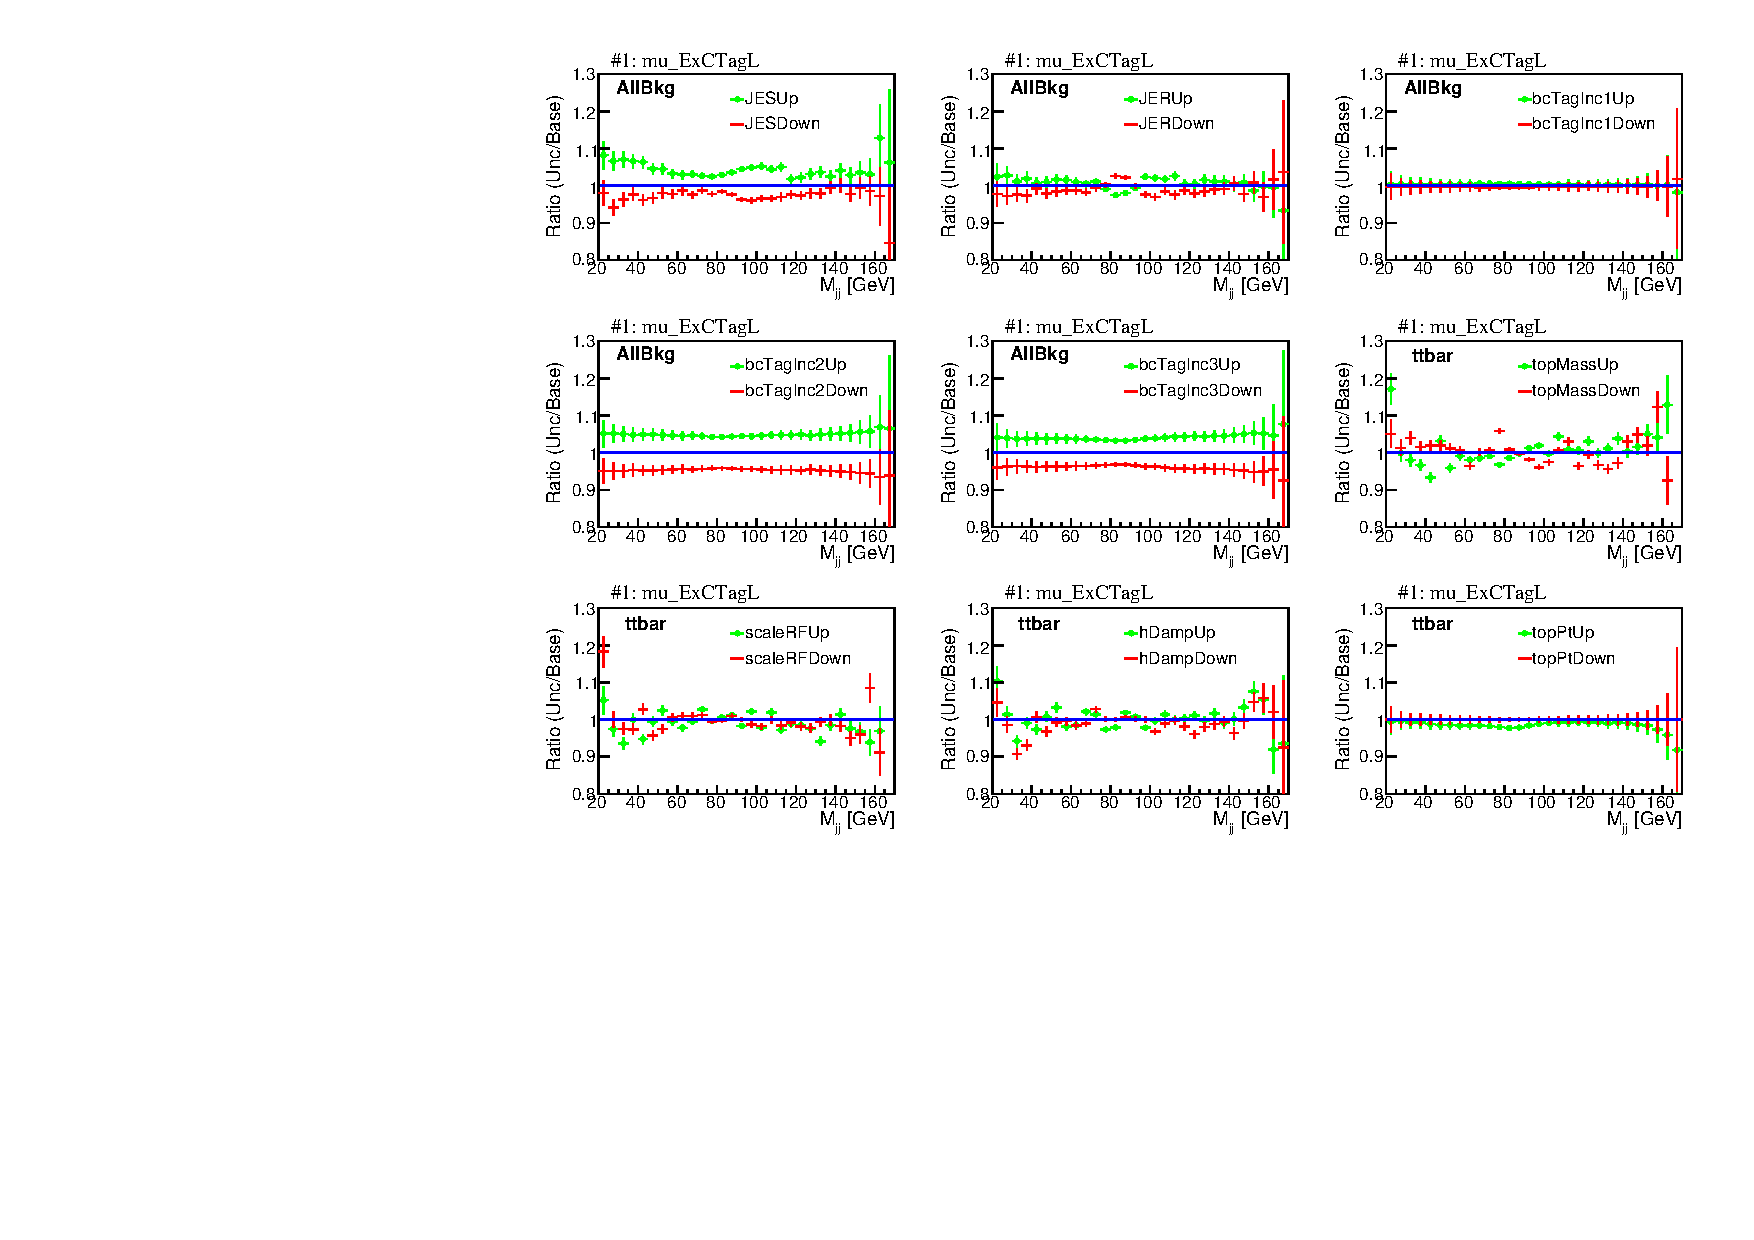
\includegraphics[width=0.95\linewidth]{Image/SYS/RatioBaseSys/mjj_1_mu_ExCTagL.pdf}}
    \caption{ Ratio of up and down with base template for exclusive loose charm category for \mujets channel. }
    \label{fig:shapeVslnN1}
\end{figure}


\begin{figure}
    \centering
    {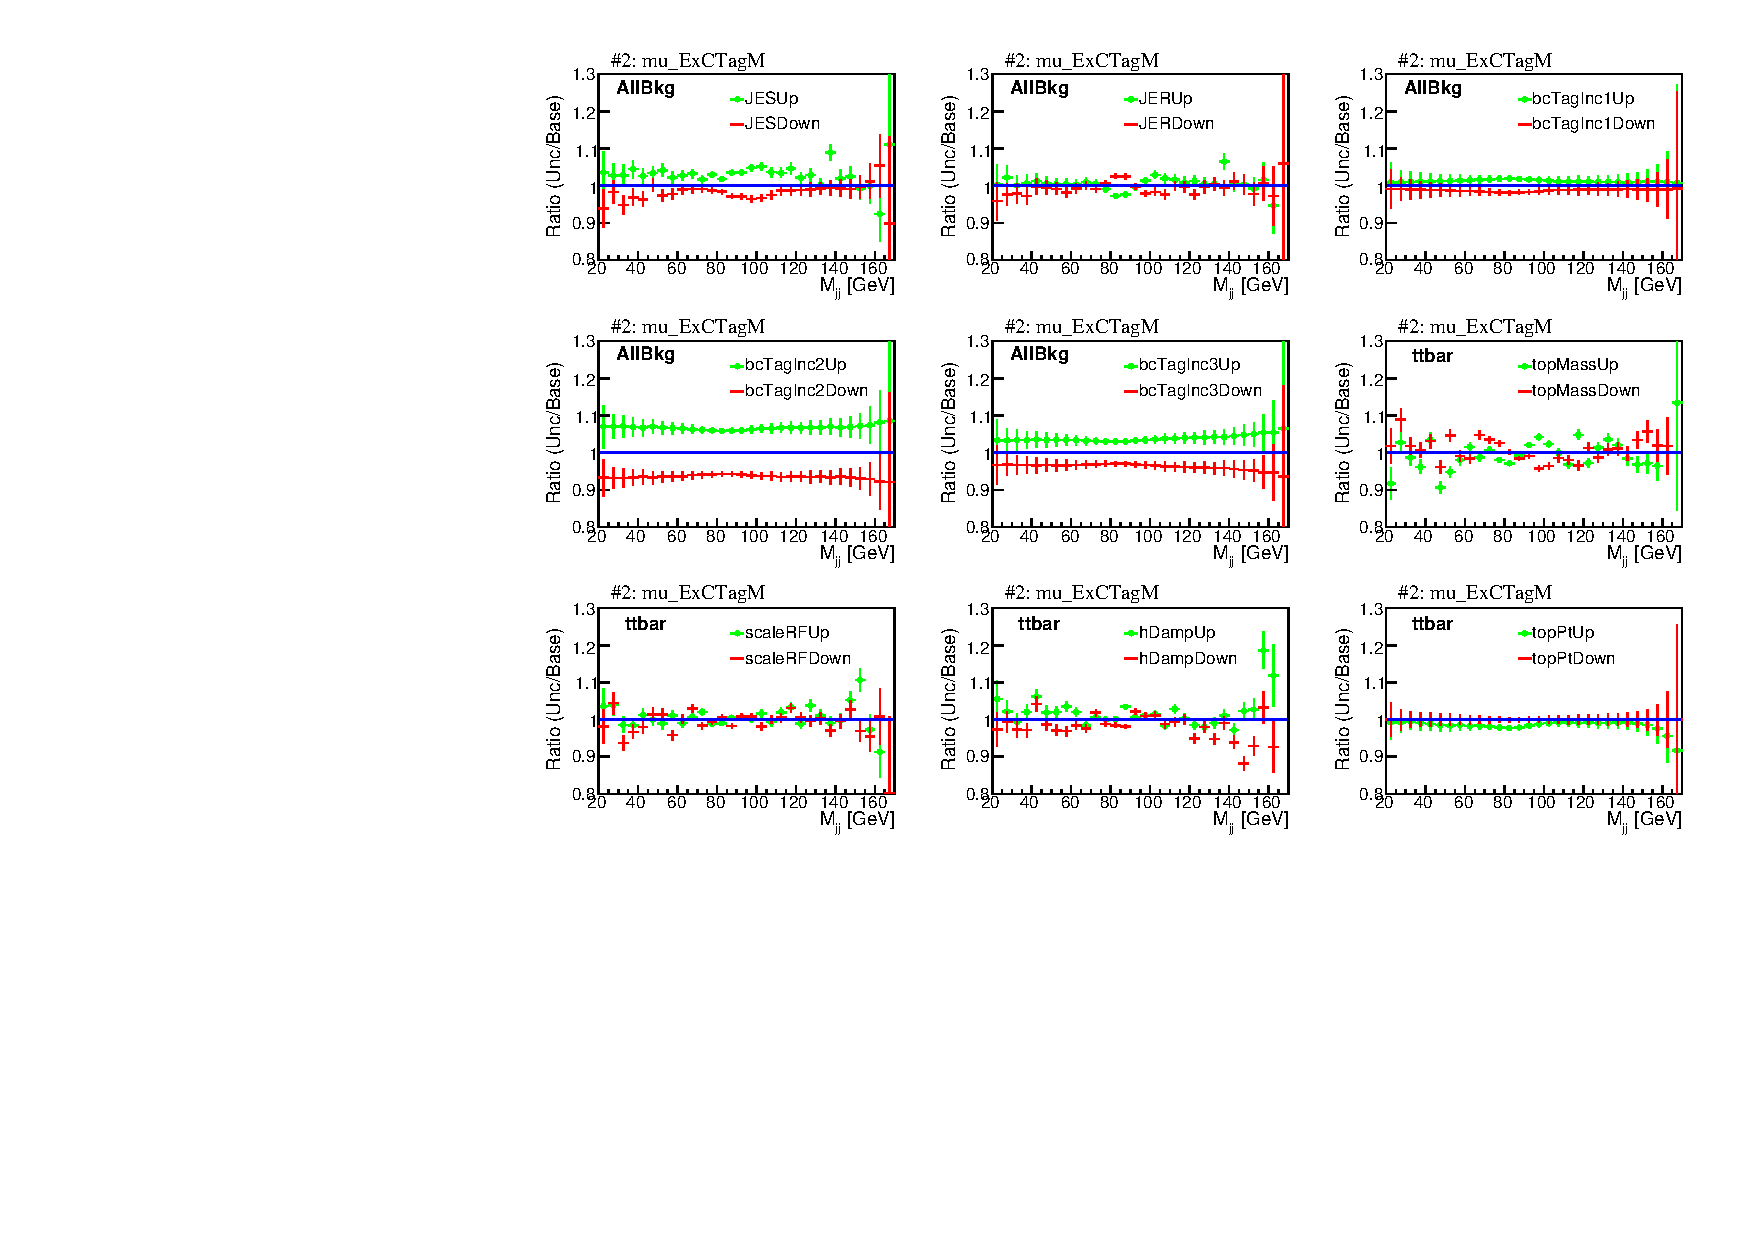
\includegraphics[width=0.95\linewidth]{Image/SYS/RatioBaseSys/mjj_2_mu_ExCTagM.pdf}}
    \caption{ Ratio of up and down with base template for exclusive medium charm category for \mujets channel.}
    \label{fig:shapeVslnN2}
\end{figure}
\begin{figure}
    \centering
    {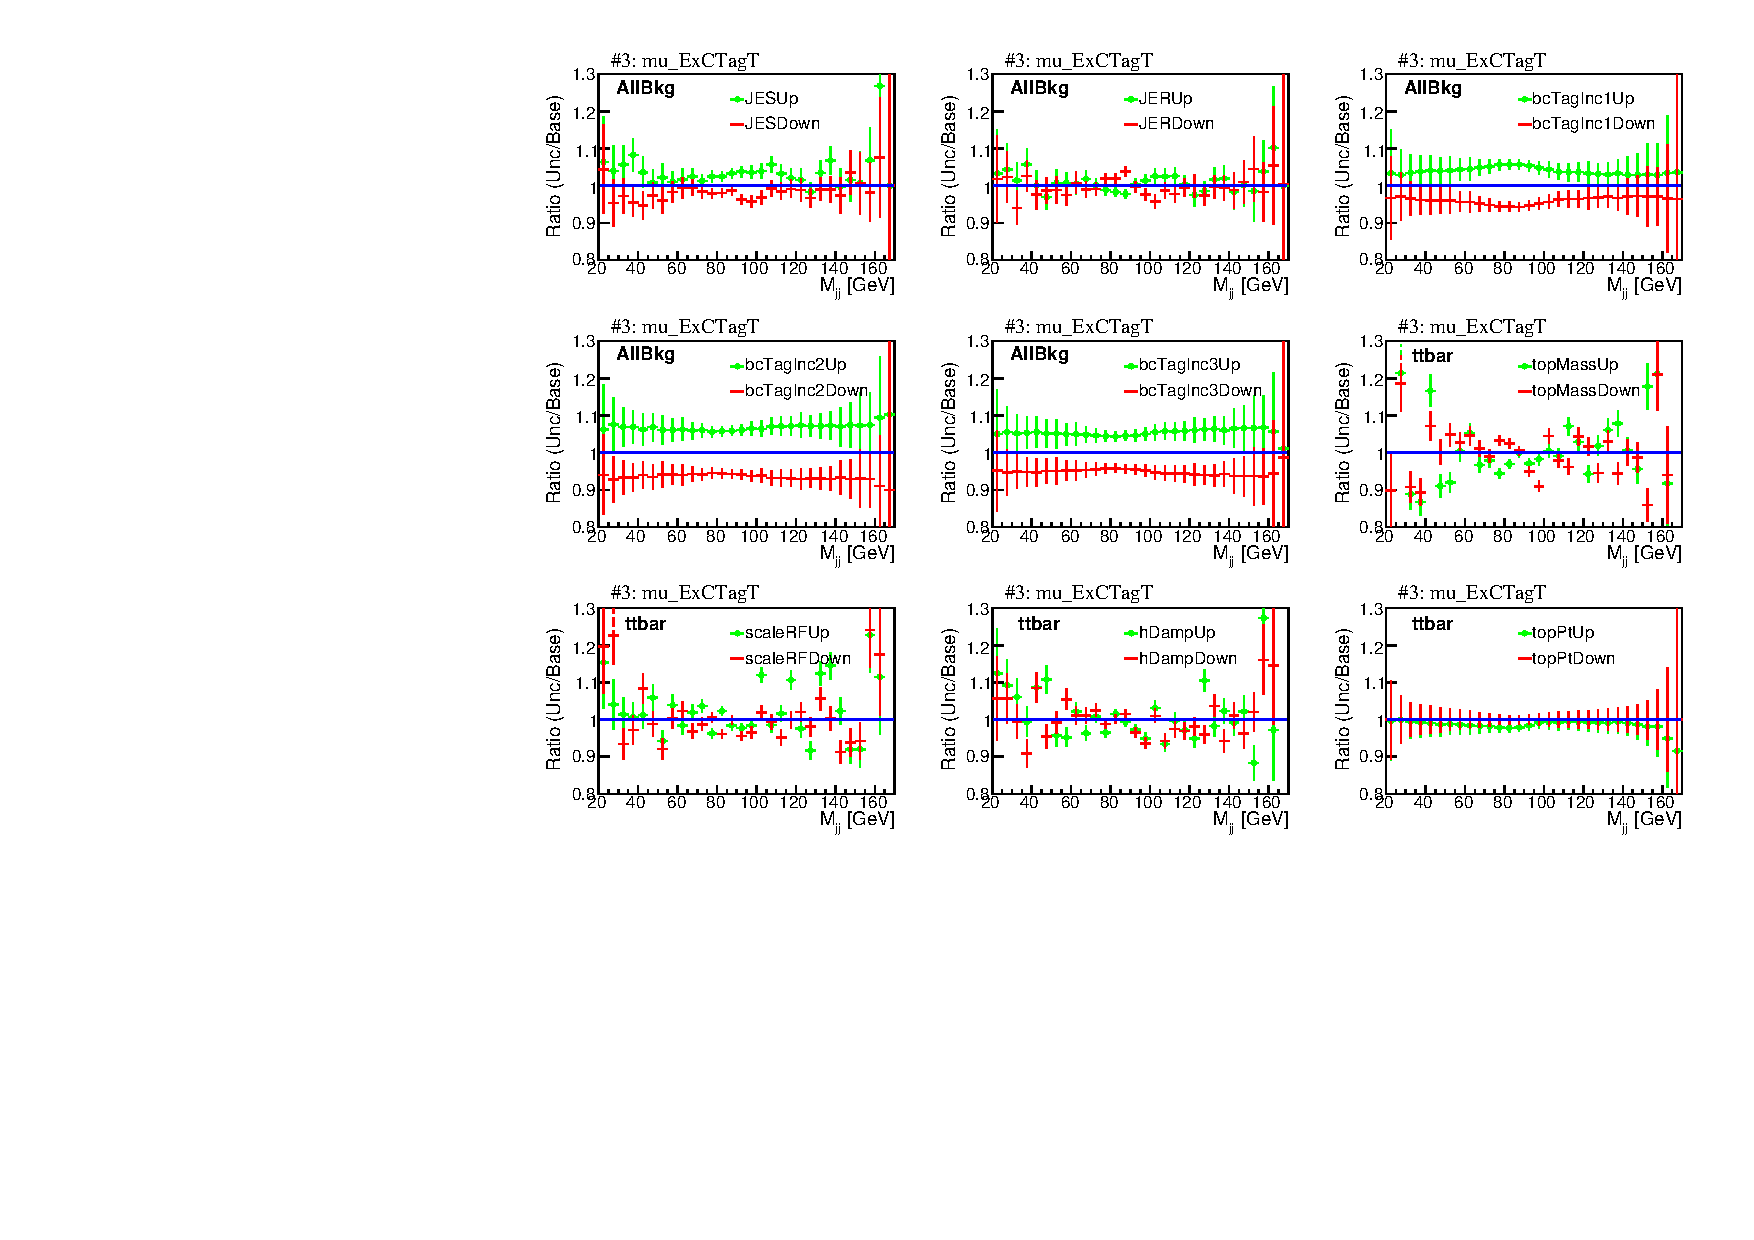
\includegraphics[width=0.95\linewidth]{Image/SYS/RatioBaseSys/mjj_3_mu_ExCTagT.pdf}}
    \caption{ Ratio of up and down with base template from  exclusive tight charm category for \mujets channel. }
    \label{fig:shapeVslnN3}
\end{figure}


\begin{figure}
    \centering
    {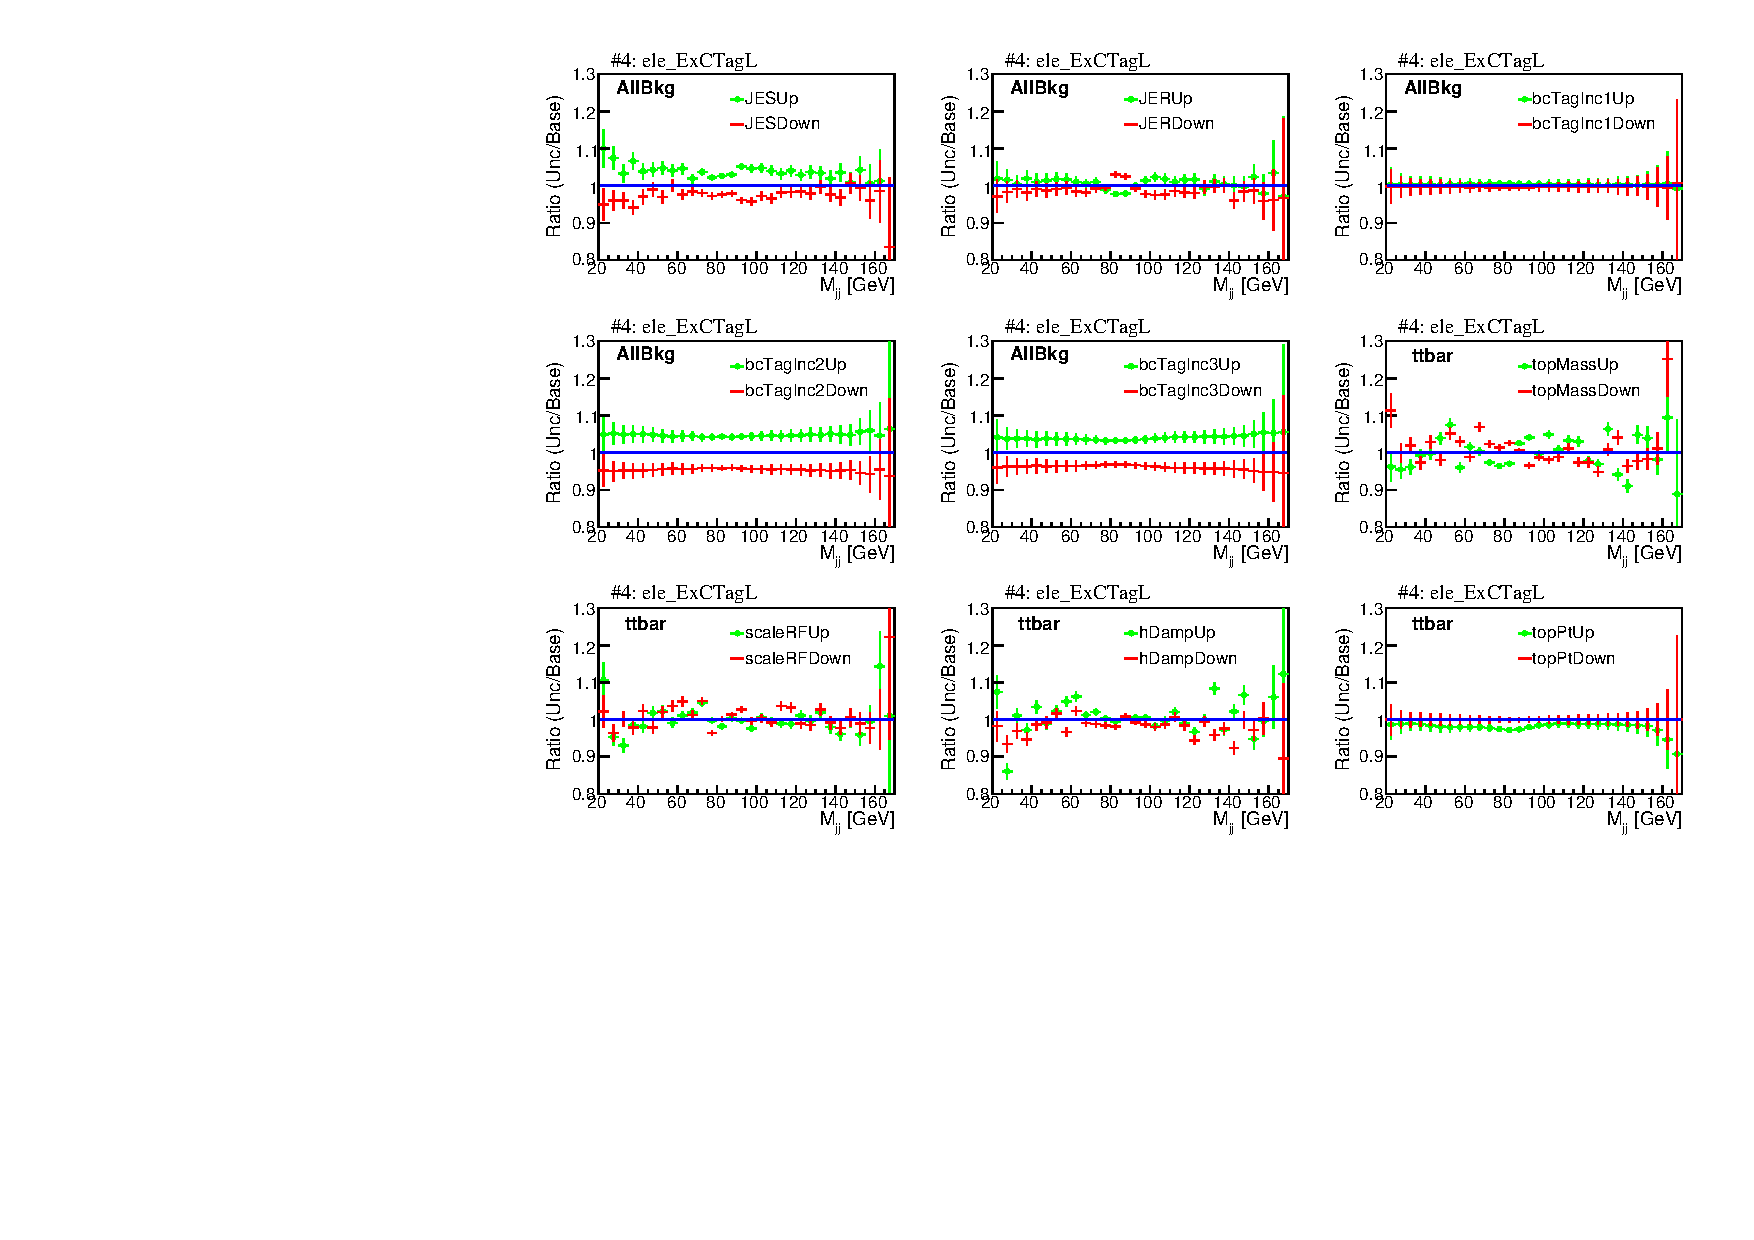
\includegraphics[width=0.95\linewidth]{Image/SYS/RatioBaseSys/mjj_4_ele_ExCTagL.pdf}}
    \caption{ Ratio of up and down with base template from exclusive loose charm category for \ejets channel.}
    \label{fig:shapeVslnN4}
\end{figure}
\begin{figure}
    \centering
    {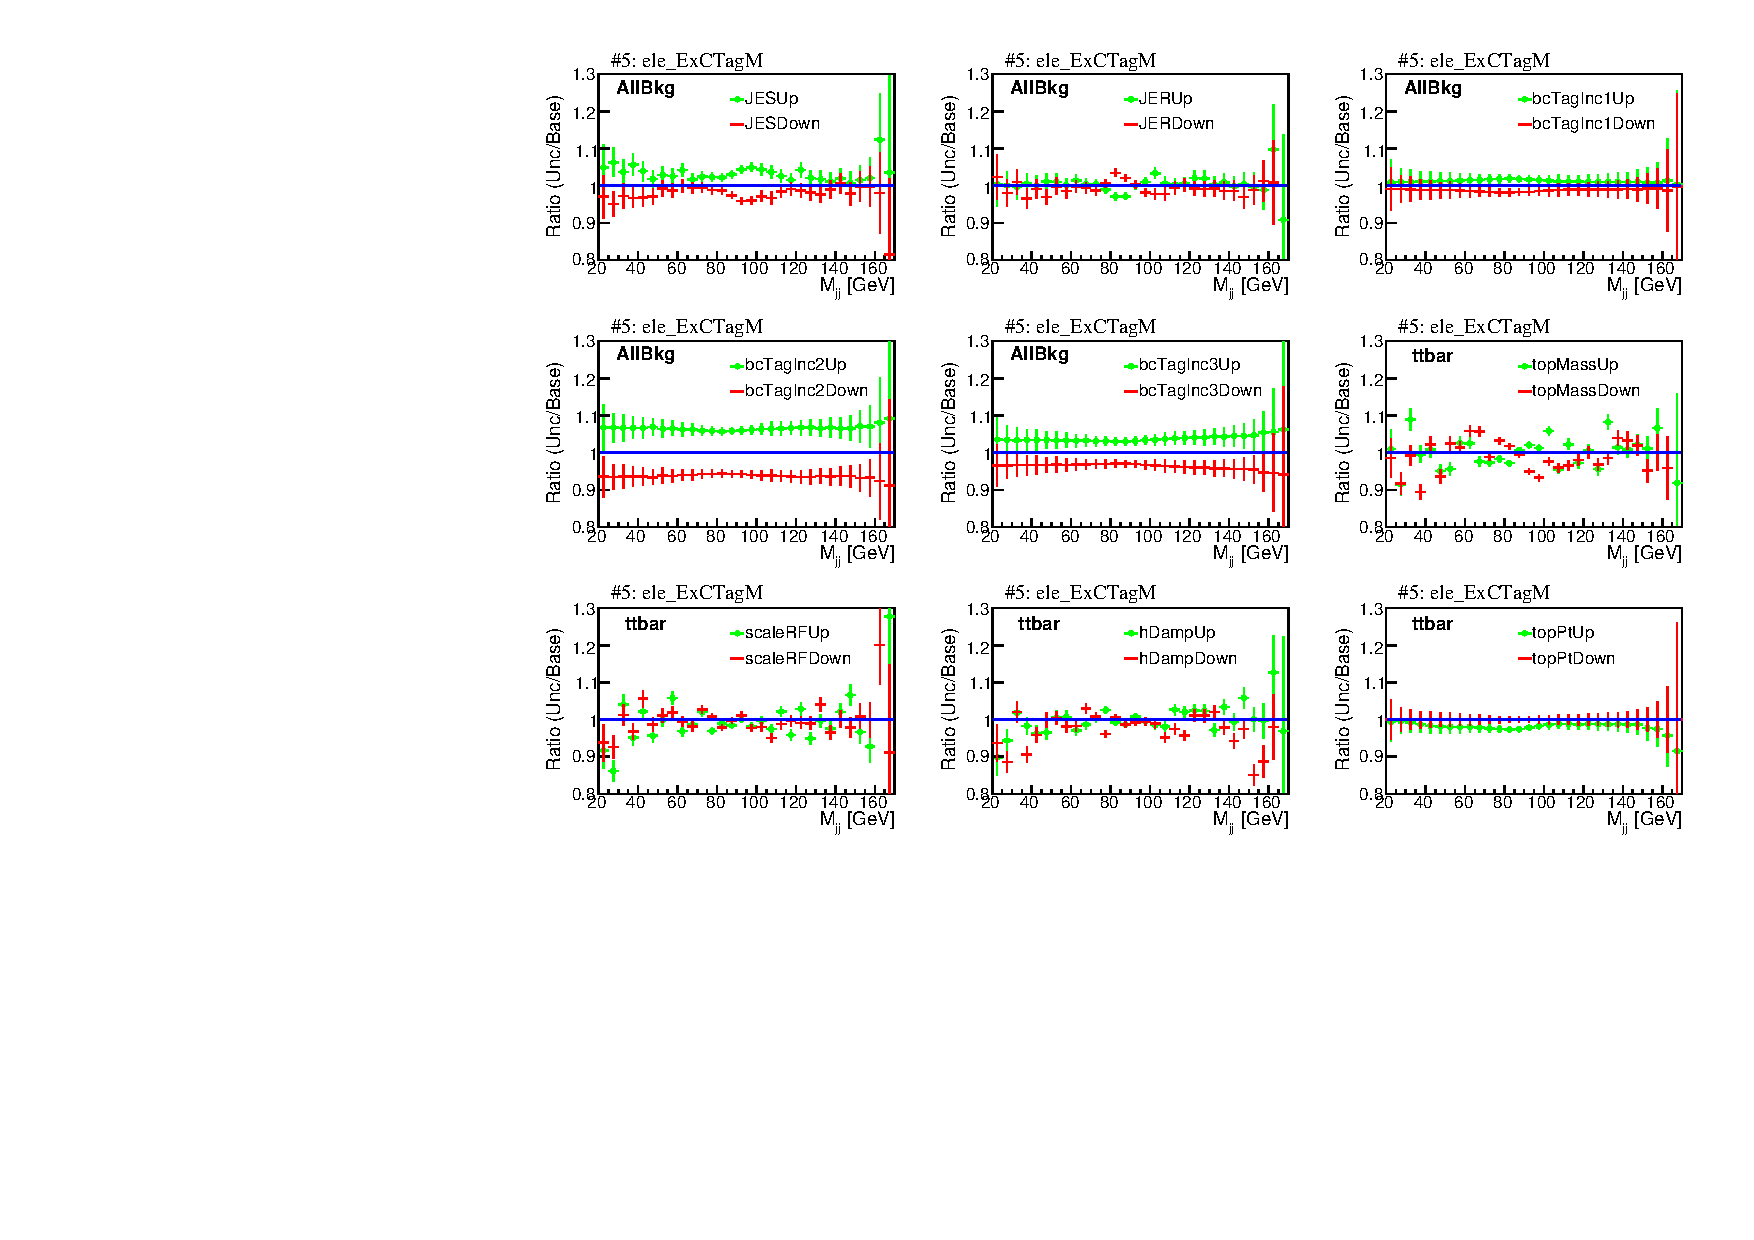
\includegraphics[width=0.95\linewidth]{Image/SYS/RatioBaseSys/mjj_5_ele_ExCTagM.pdf}}
    \caption{ Ratio of up and down with base template from exclusive medium charm category for \ejets channel. }
    \label{fig:shapeVslnN5}
\end{figure}


\begin{figure}
    \centering
    {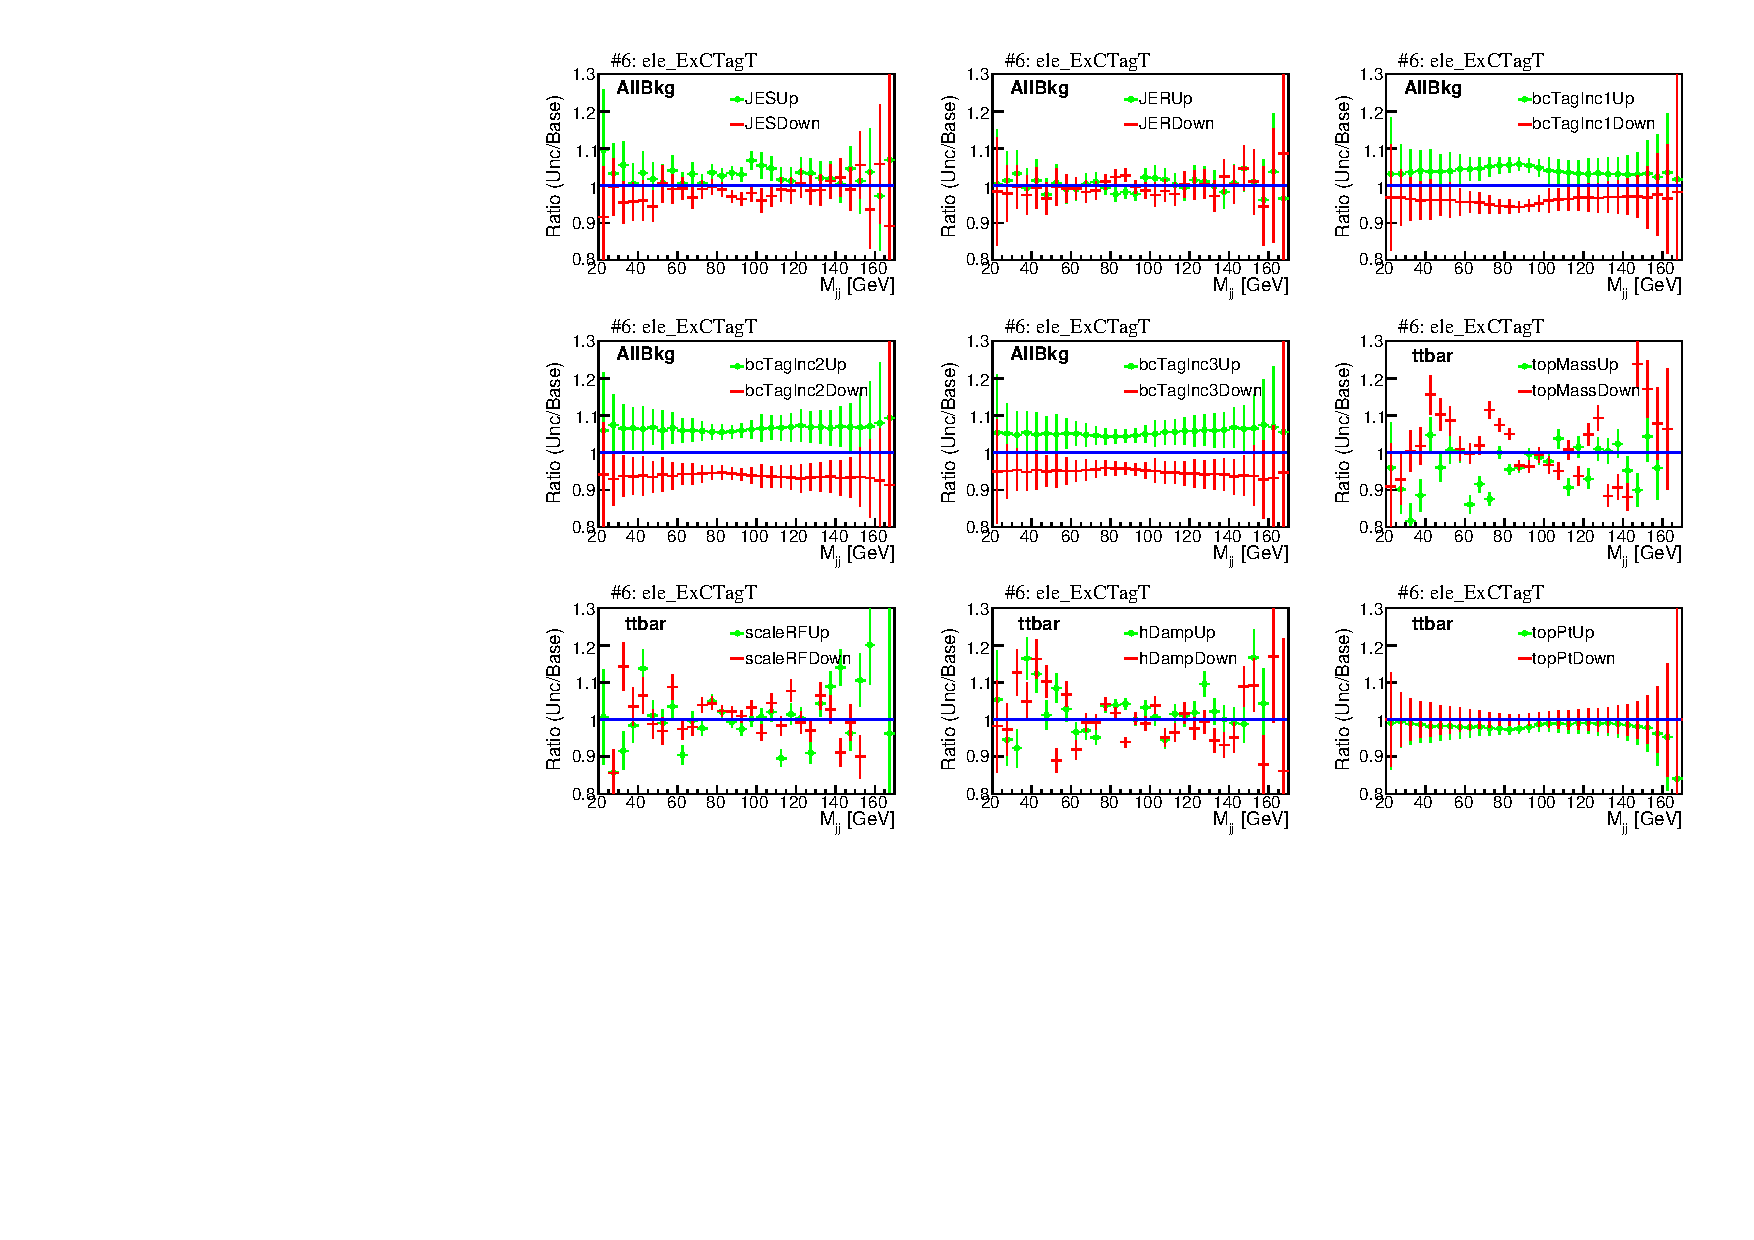
\includegraphics[width=0.95\linewidth]{Image/SYS/RatioBaseSys/mjj_6_ele_ExCTagT.pdf}}
    \caption{ Ratio of up and down with base template from exclusive tight charm category for \ejets channel.}
    \label{fig:shapeVslnN6}
\end{figure}


\subsection{Distributions of Pulls}
A maximum likelihood fit is performed on the data. After the fit, the
background yield as well as uncertainties are changed so that the backgrounds
fit well with the data. The extent of change in the individual uncertainty
is shown in Figures~\ref{fig:fitDiag1}-\ref{fig:fitDiag4} for lepton channel for
charged Higgs mass 100 GeV. In these figures, the error bars on the left-hand
side represents the ratio of post (after the background-only) and pre-fit
(prior to the fit to data) uncertainty. If the length of the error bar is small
(say 0.80) then the post-fit uncertainty is reduced (by 20\%). On the right
hand side of the plot, the correlation between the BR and ncertainty is shown.
From these figures, one can see that the NPs from autoMCStats have almost no
correlation with BR. The background-only fit is obtained by setting the signal
strength to zero. The signal+ background fit is obtained by using floating
signal strength. The distributions of pulls are produced using the Command (\ref{cmd:fitDiag}).
\begin{table}
\begin{center}
\begin{tabular}{ccc}
\hline
\hline
{\bf{Acronym}} & {\bf{channel}} & {\bf{Event category}}\\
\hline
\hline
binch1    & \mujets     & exclusive loose\\
binch2    & \mujets     & exclusive medium\\
binch3    & \mujets     & exclusive tight\\
binch4    & \ejets & exclusive loose\\
binch5    & \ejets & exclusive medium\\
binch6    & \ejets & exclusive tight\\
\hline
\end{tabular}
\caption{Acronym used in the autoMCStat tool for naming nuisance parameters.}.
\end{center}
\label{tab:autoMCStat}
\end{table}


\begin{figure}
\begin{center}
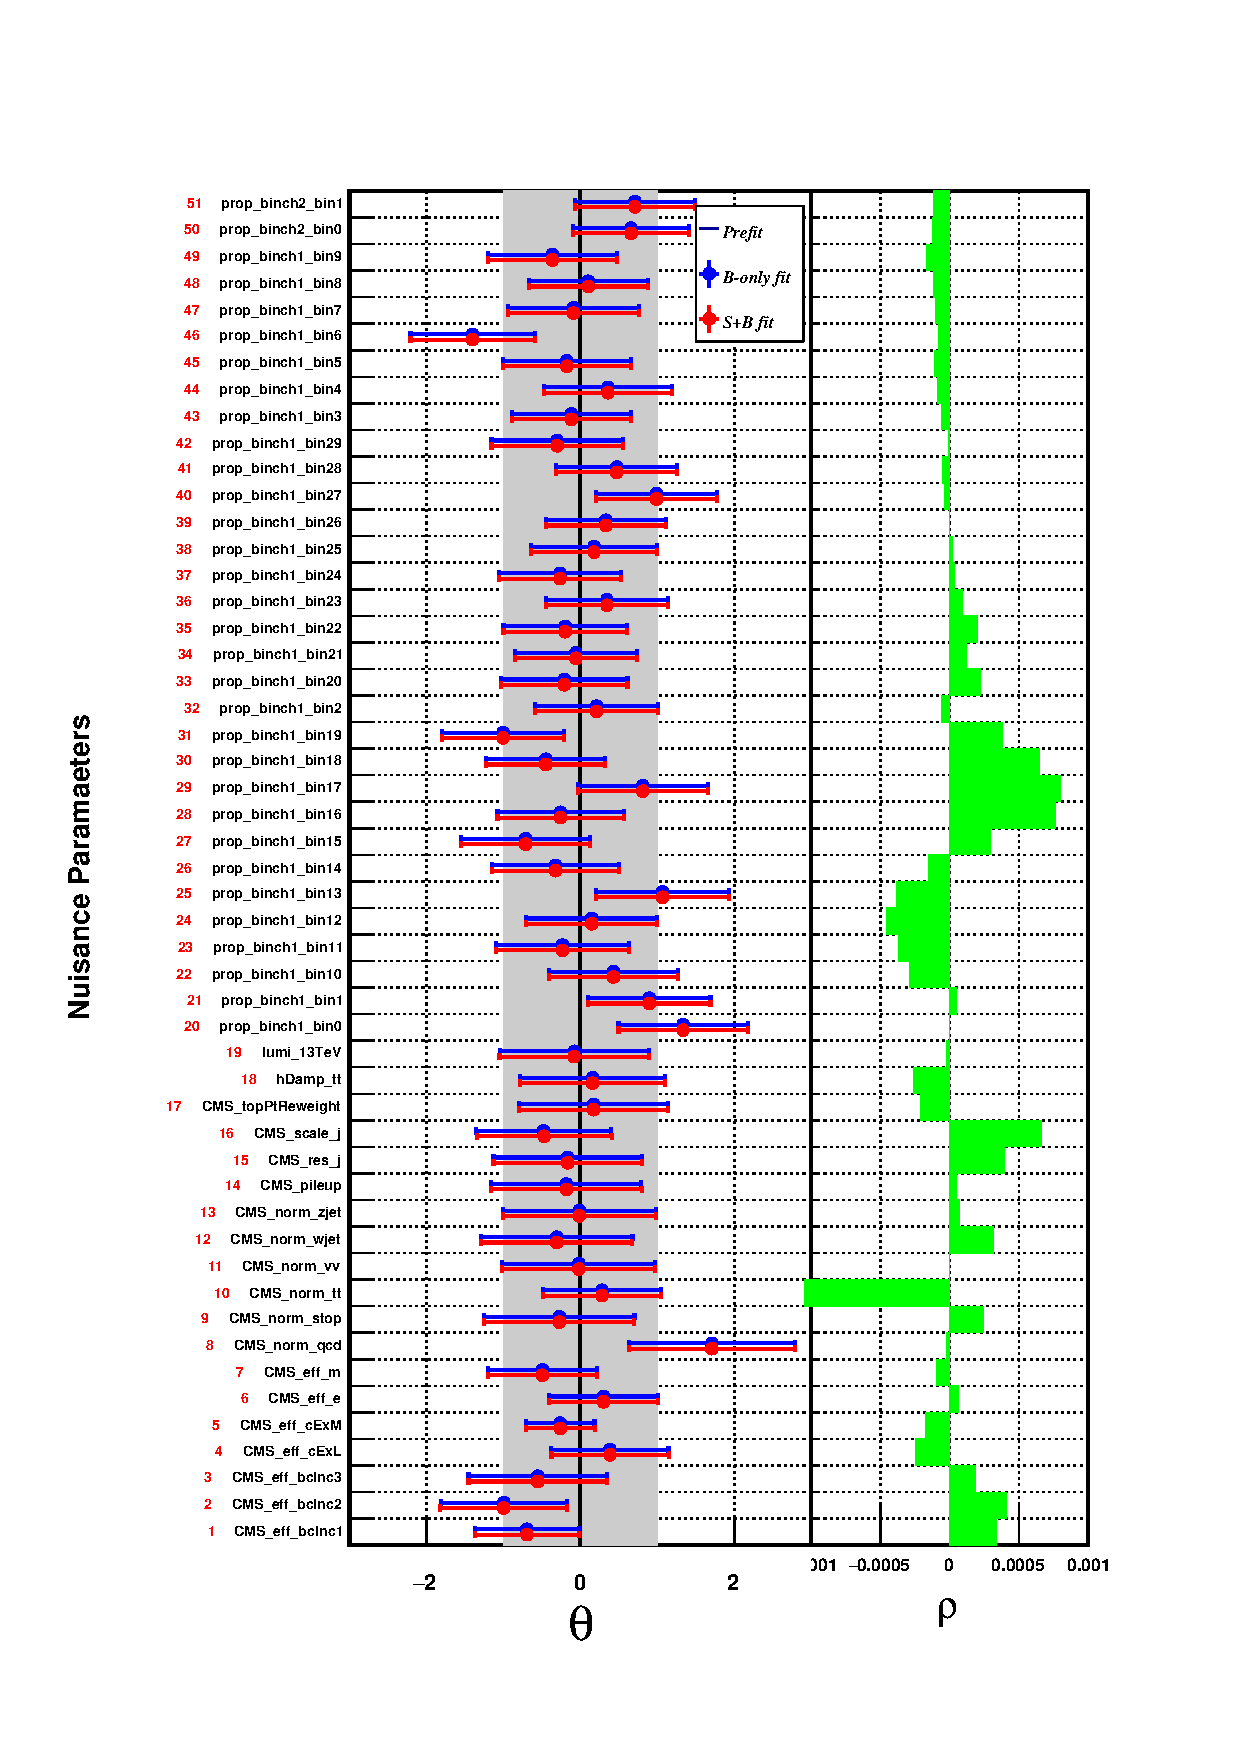
\includegraphics[width=1.0\textwidth]{Image/MLFit/FitDiag/fitDiag1.pdf}
 \caption{Output of the $FitDiagnostics$ using \mjj from
     exclusive event categories based on charm-tagging for $m_{H^+} = 100$
     GeV from \ljets channel. The pre-fit value $\theta_0 = 0$ and the uncertainty on the
     pre-fit value $\Delta\theta = 1$. The $\rho$ is the correlation between NPs and $BR$. Contd ...}
\label{fig:fitDiag1}
\end{center}
\end{figure}

\begin{figure}
\begin{center}
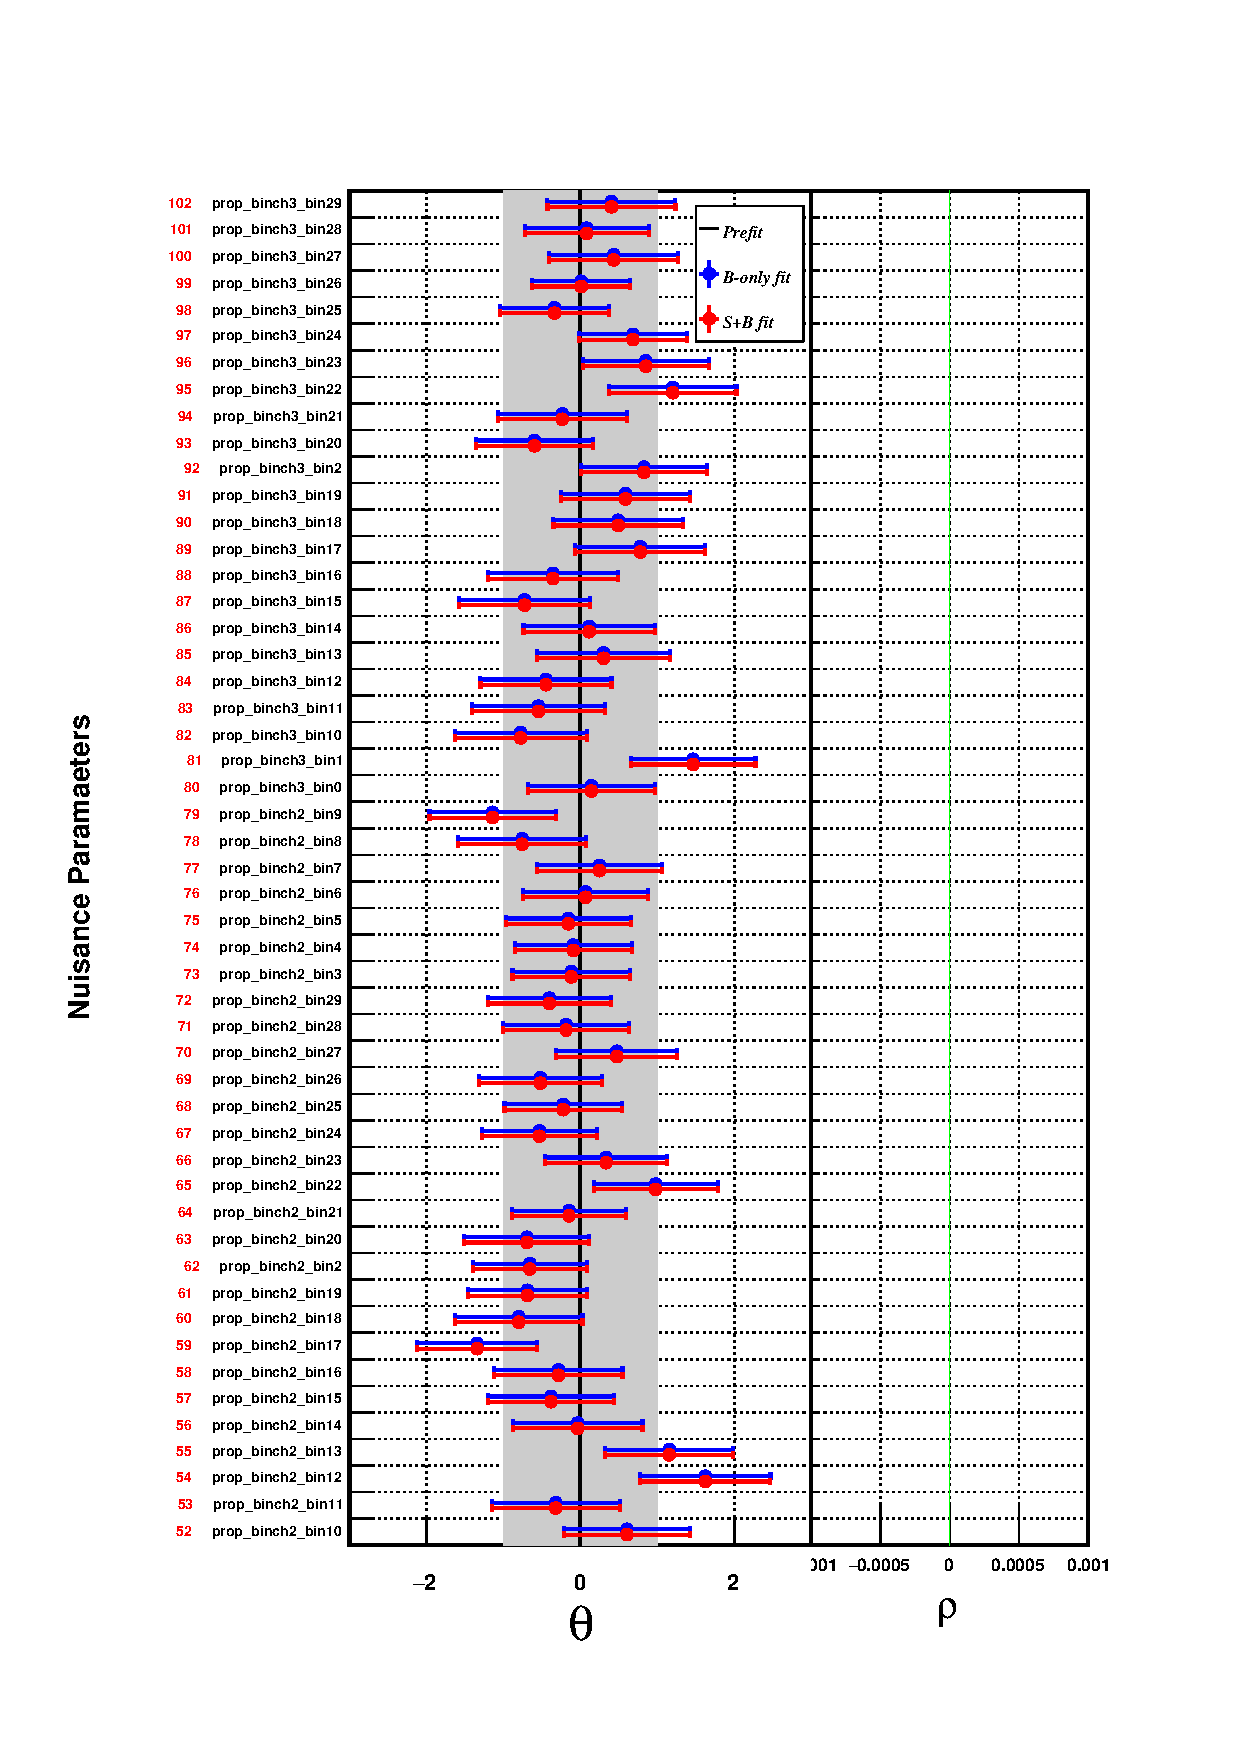
\includegraphics[width=1.0\textwidth]{Image/MLFit/FitDiag/fitDiag2.pdf}
 \caption{Output of the $FitDiagnostics$ using \mjj from
     exclusive event categories based on charm-tagging for $m_{H^+} = 100$
     GeV from \ljets channel. The pre-fit value $\theta_0 = 0$ and the uncertainty on the
     pre-fit value $\Delta\theta = 1$. The $\rho$ is the correlation between NPs and $BR$. Contd ...}
\label{fig:fitDiag2}
\end{center}
\end{figure}

\begin{figure}
\begin{center}
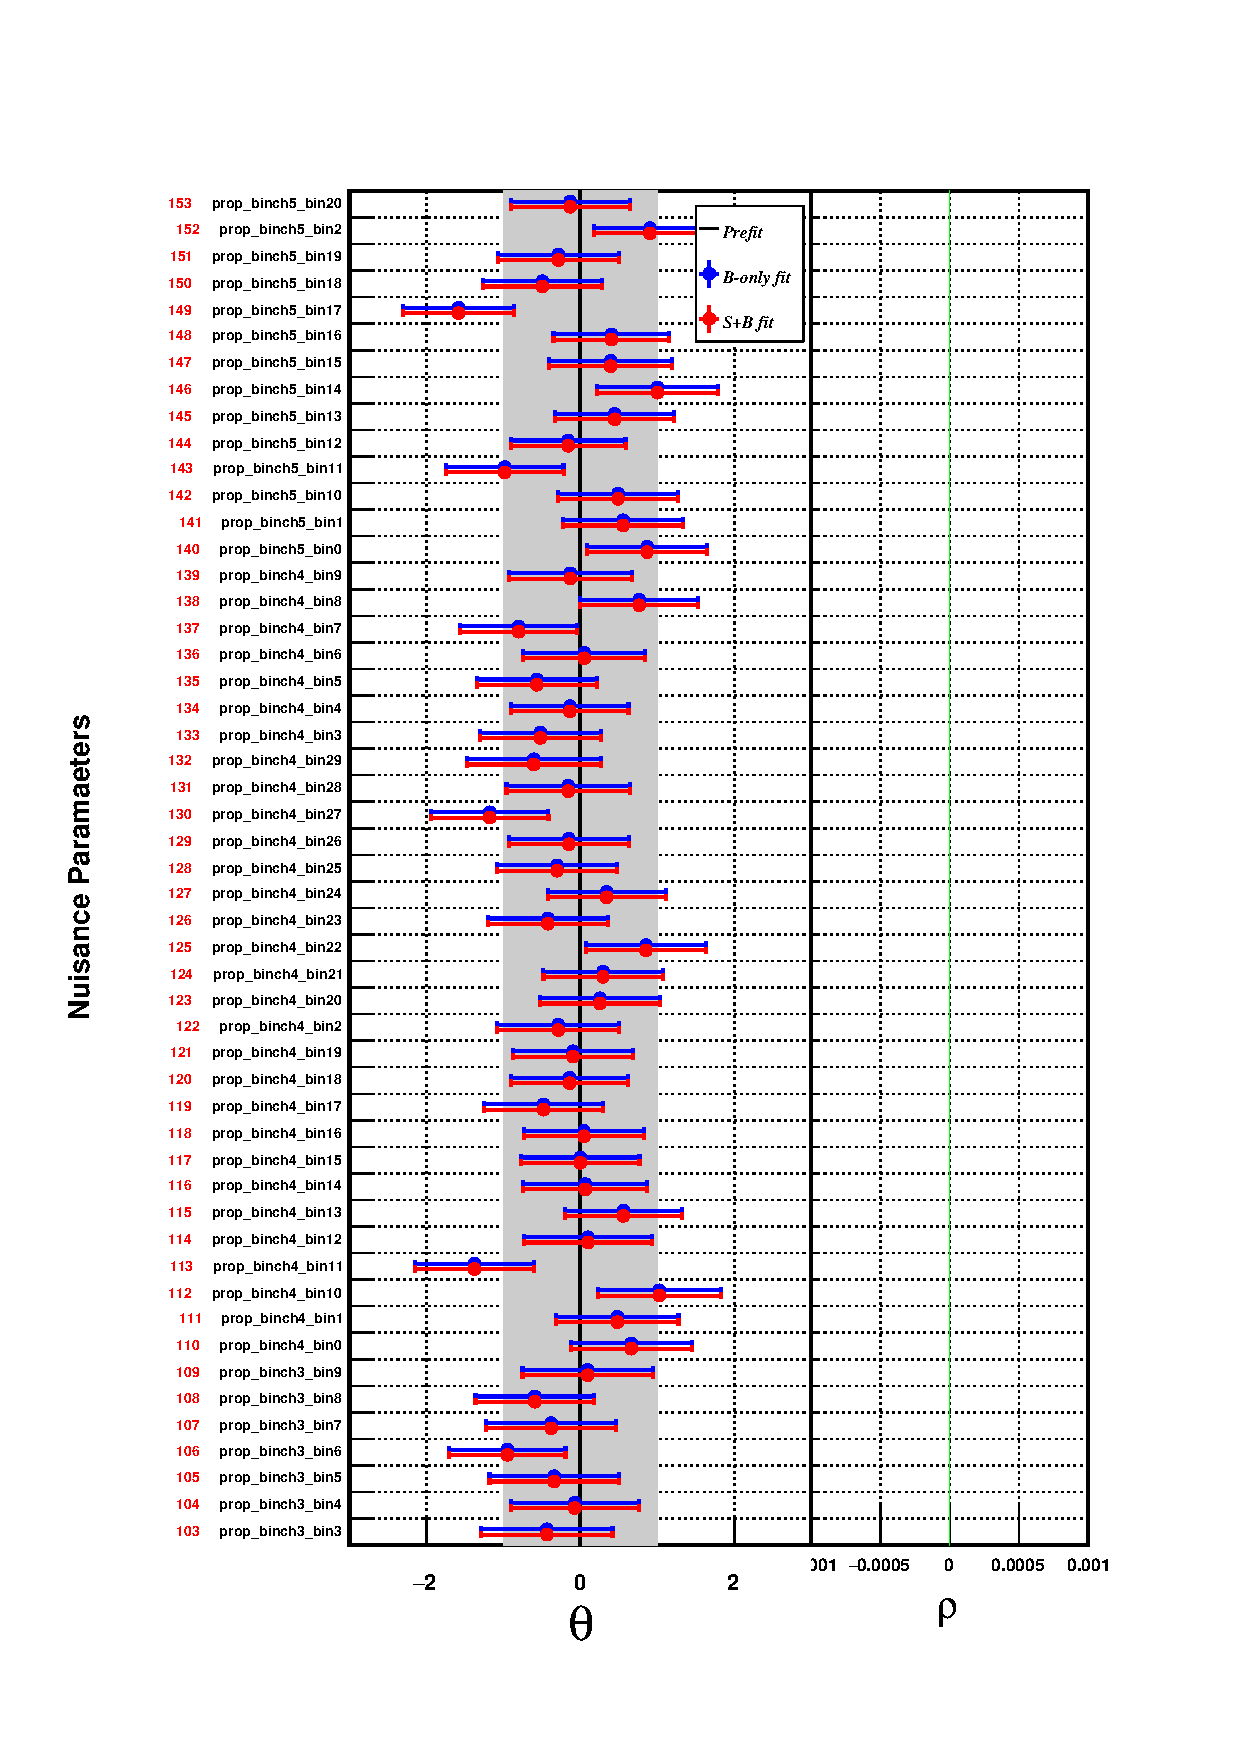
\includegraphics[width=1.0\textwidth]{Image/MLFit/FitDiag/fitDiag3.pdf}
 \caption{Output of the $FitDiagnostics$ using \mjj from
     exclusive event categories based on charm-tagging for $m_{H^+} = 100$
     GeV from \ljets channel. The pre-fit value $\theta_0 = 0$ and the uncertainty on the
     pre-fit value $\Delta\theta = 1$. The $\rho$ is the correlation between NPs and $BR$. Contd ...}
\label{fig:fitDiag3}
\end{center}
\end{figure}

\begin{figure}
\begin{center}
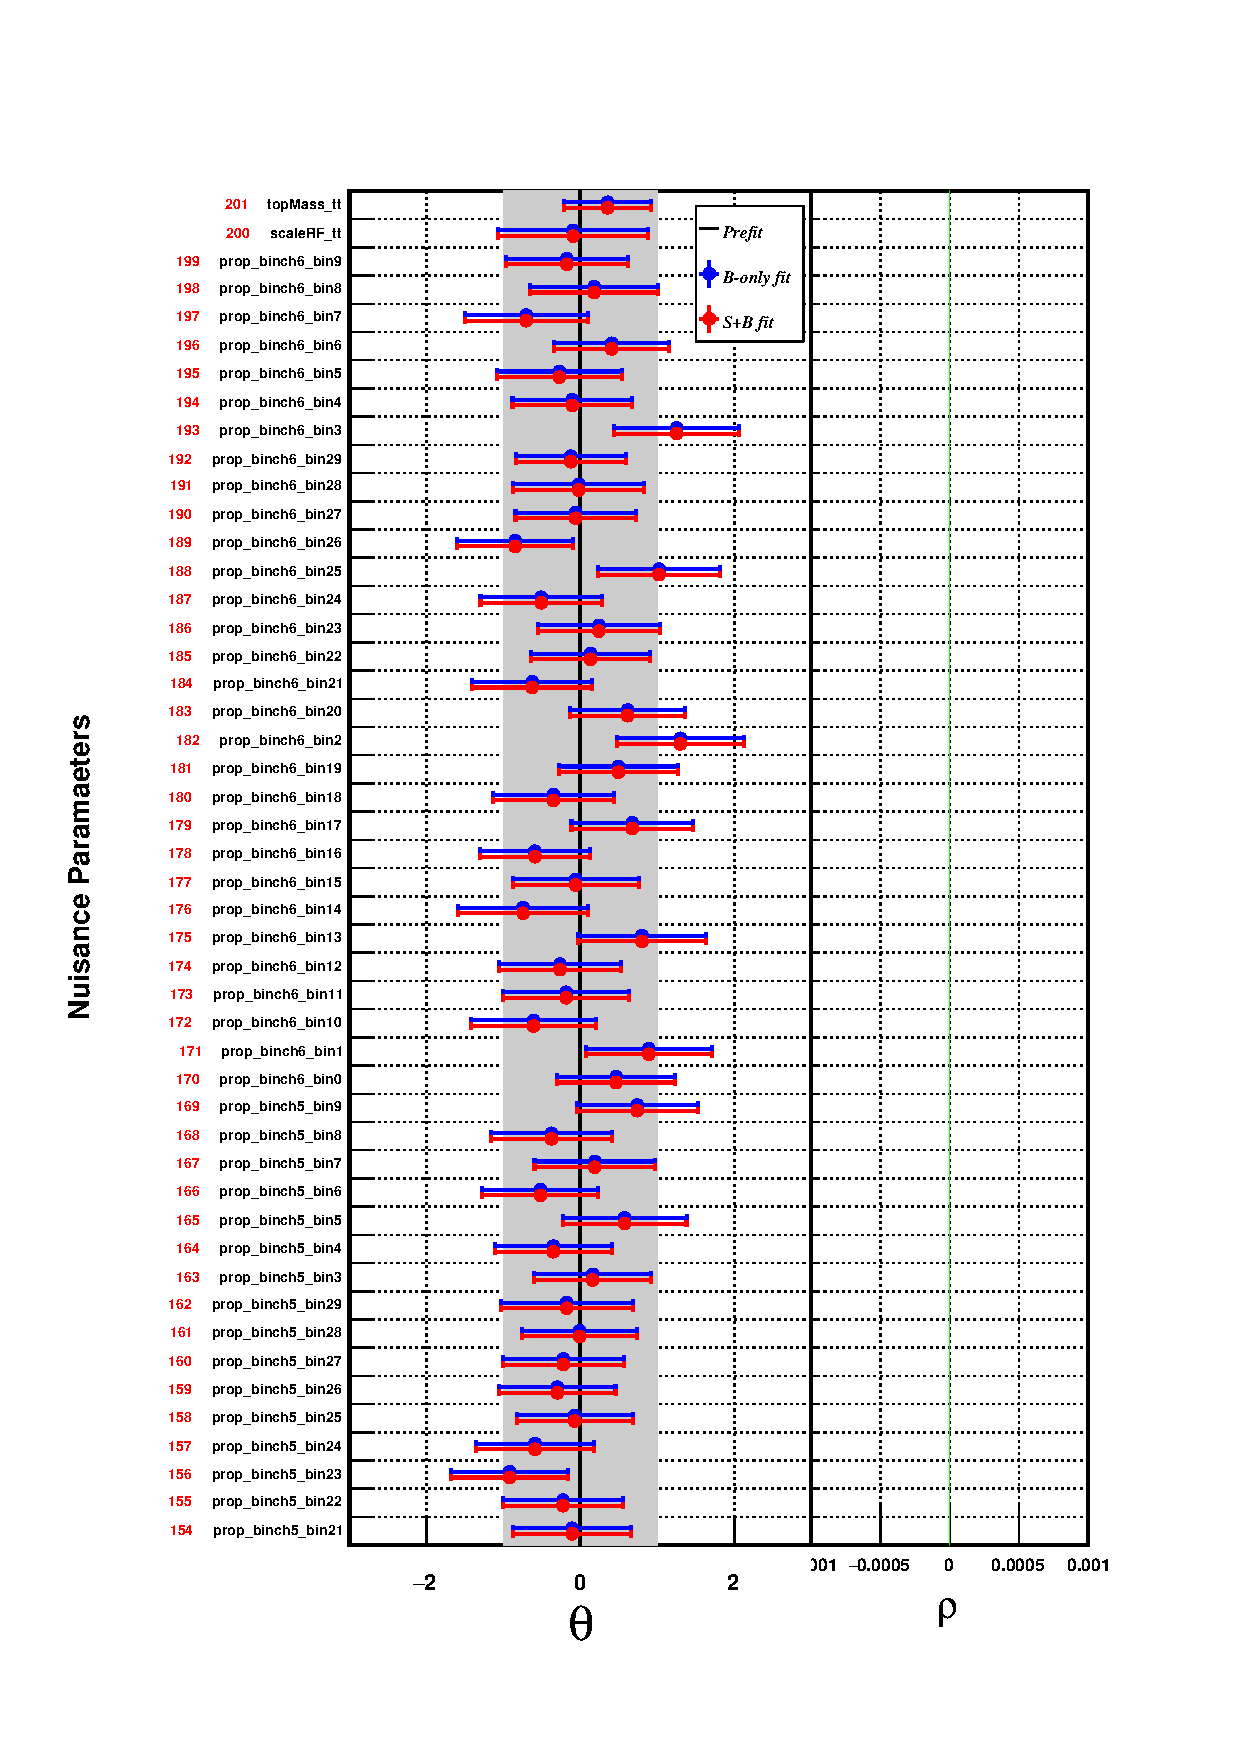
\includegraphics[width=1.0\textwidth]{Image/MLFit/FitDiag/fitDiag4.pdf}
 \caption{Output of the $FitDiagnostics$ using \mjj from
     exclusive event categories based on charm-tagging for $m_{H^+} = 100$
     GeV from \ljets channel. The pre-fit value $\theta_0 = 0$ and the uncertainty on the
     pre-fit value $\Delta\theta = 1$. The $\rho$ is the correlation between NPs and $BR$.}
\label{fig:fitDiag4}
\end{center}
\end{figure}

\subsection{Post-fit Yields and Distributions}
The event yields, after a background-only fit to the data, of all the background
process for both channels from all charm-tagging categories are shown in
Table~\ref{tab:eventYieldPost}. The corresponding $\mjj$ distributions are shown
in Figure~\ref{fig:mjjPostFit}. From these plots, one can see that the uncertainty
band is reduced. Which indicates that the fit has reduced the uncertainties.
Since the SM $\ttjets$ is the dominant background, the pre-fit and post-fit
distribution of this process is shown in Figure~\ref{fig:ttbarPostFit} to gauge
the change after the fit. From this figure, one can also see that the post-fit
yields are getting reduced as one goes from loose to the tight charm-category.
\begin{table}
  \centering
\caption{Expected event yields for background processes, after a background-only
    fit to the data, in each of the channels and event category. The number of
    events, along with the uncertainty (including statistical and systematic effects),
    is shown.}
\label{tab:eventYieldPost}
\begin{adjustbox}{max width=\textwidth}
\begin{tabular}{cccccccc}
\hline
\hline
\multicolumn{1}{c}{{\bf{Process}}} & \multicolumn{2}{c}{{Loose}} & \multicolumn{2}{c}{{Medium}} & \multicolumn{2}{c}{{Tight}} \\
                  & $\mu$ + jets   &  e + jets      & $\mu$ + jets   &  e + jets      & $\mu$ + jets   &  e + jets \\
\hline
\hline
SM $\ttbar$ + jets & 100537 $\pm$ 410 & 71803 $\pm$ 473 & 73211 $\pm$ 320 & 52340 $\pm$ 288 & 18762 $\pm$ 134 & 13376 $\pm$ 127 \\ 
Single \PQt & 2747 $\pm$ 215 & 1968 $\pm$ 162 & 1939 $\pm$ 155 & 1397 $\pm$ 114 & 421 $\pm$ 35 & 302 $\pm$ 26 \\ 
QCD multijet & 517 $\pm$ 130 & 2123 $\pm$ 468 & 498 $\pm$ 98 & 1456 $\pm$ 213 & 88 $\pm$ 28 & 346 $\pm$ 39 \\ 
\PW + jets & 1359 $\pm$ 139 & 1061 $\pm$ 90 & 948 $\pm$ 110 & 681 $\pm$ 58 & 127 $\pm$ 23 & 102 $\pm$ 9 \\ 
$\PZ/\PGg$ + jets & 189 $\pm$ 18 & 240 $\pm$ 25 & 132 $\pm$ 13 & 132 $\pm$ 14 & 56 $\pm$ 7 & 31 $\pm$ 4 \\ 
VV & 61 $\pm$ 9 & 43 $\pm$ 6 & 56 $\pm$ 8 & 11 $\pm$ 4 & 15 $\pm$ 5 & 3 $\pm$ 1 \\ 
\hline
All background & 105410 $\pm$ 501 & 77238 $\pm$ 692 & 76784 $\pm$ 386 & 56017 $\pm$ 381 & 19469 $\pm$ 144 & 14160 $\pm$ 136 \\ 
\hline
Data & 105474 & 77244 & 76807 & 56051 & 19437 & 14179 \\
\hline
\end{tabular}
\end{adjustbox}
\end{table}
\begin{figure}
\centering
{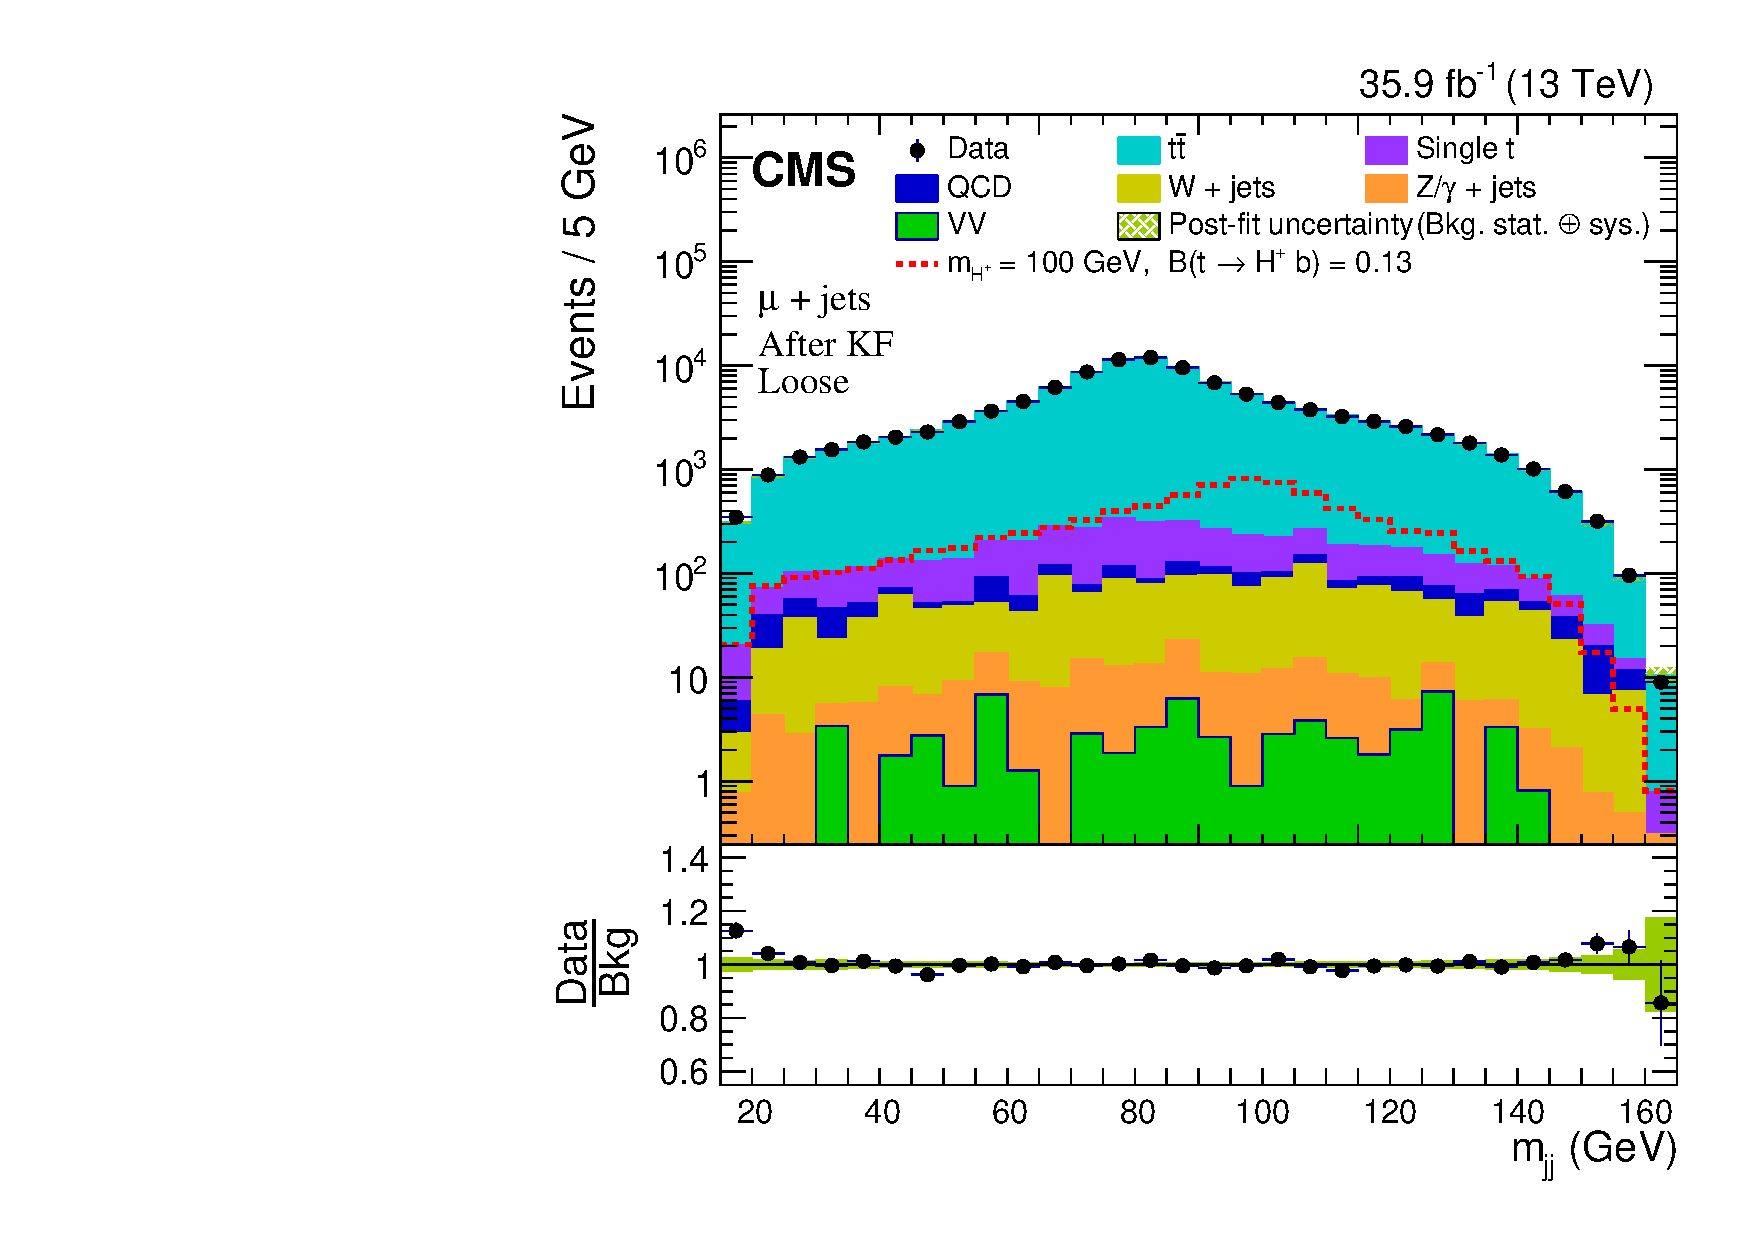
\includegraphics[width=0.45\textwidth]{Image/PostFit/mjj_postfit_ch1.pdf}}
{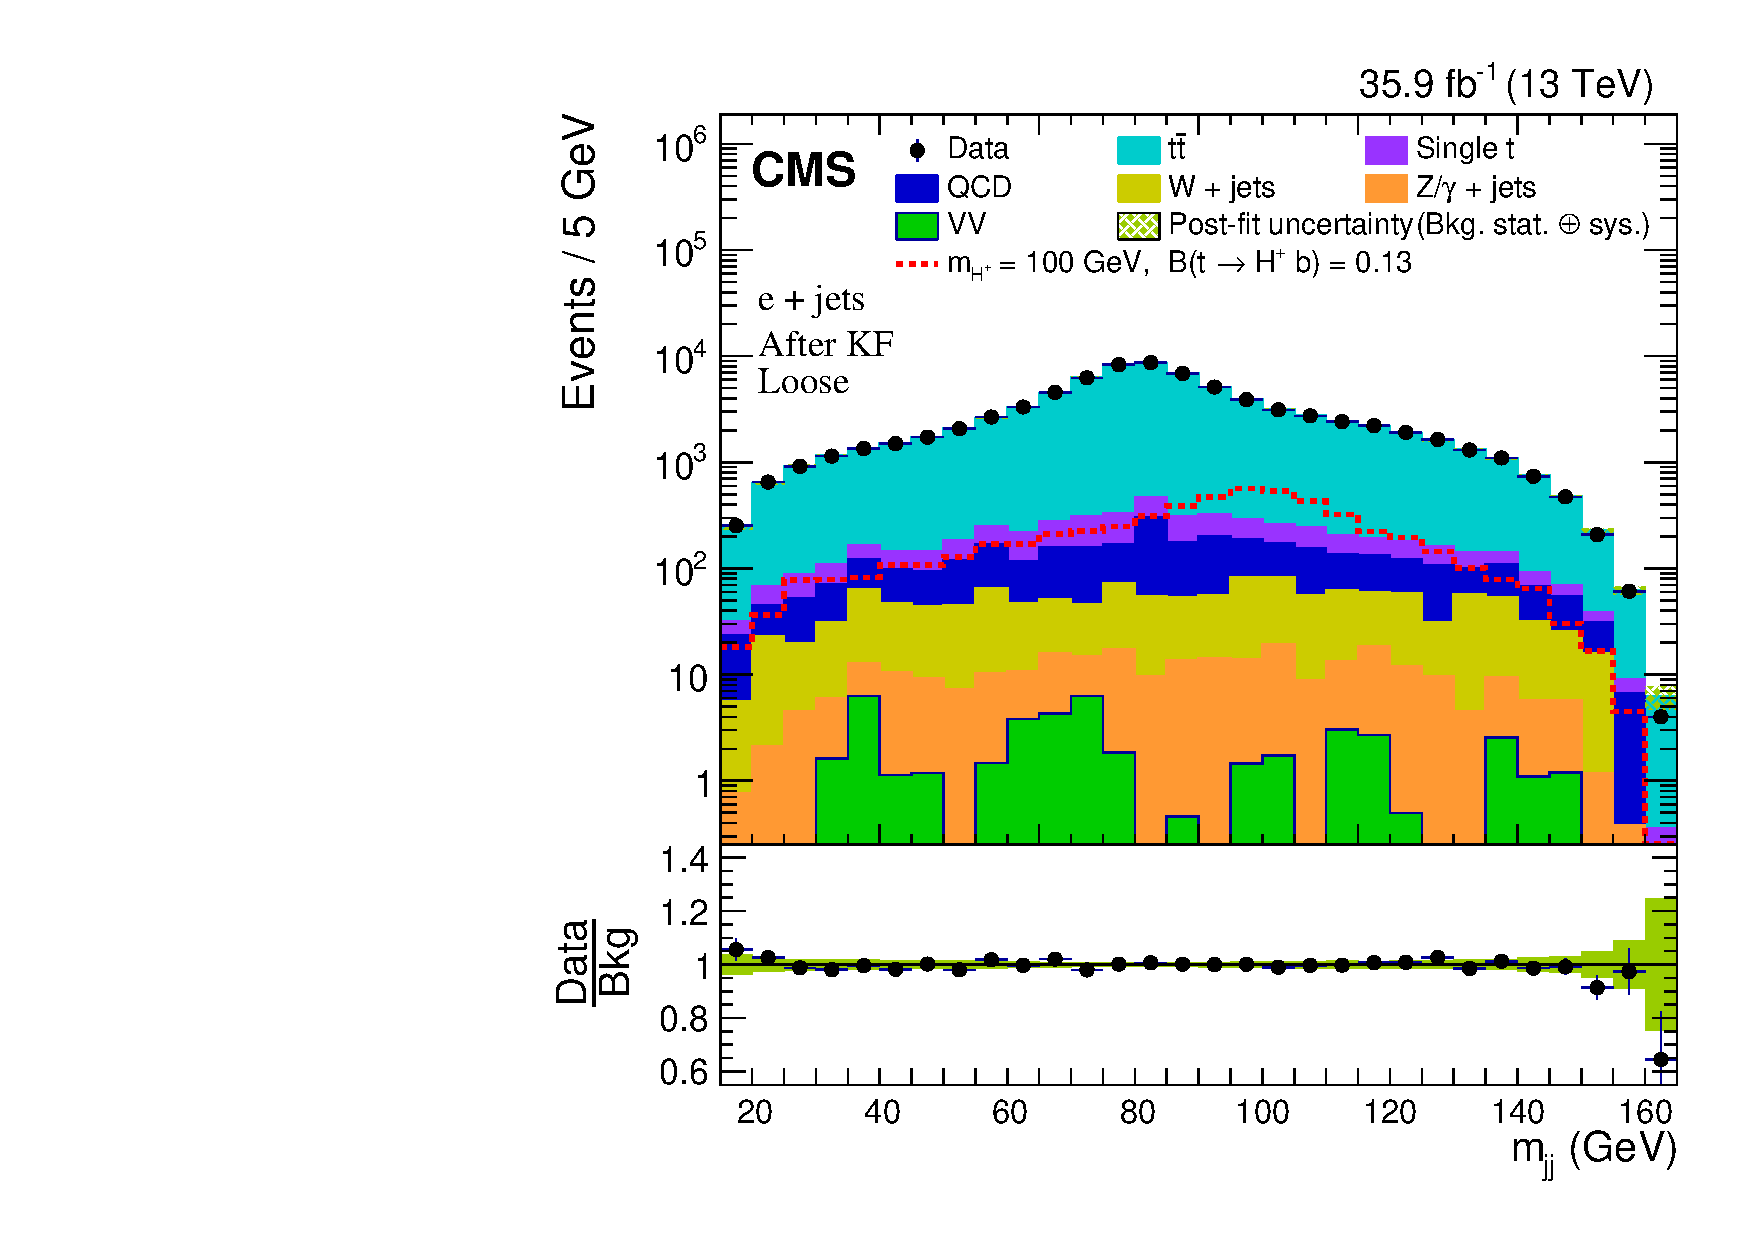
\includegraphics[width=0.45\textwidth]{Image/PostFit/mjj_postfit_ch4.pdf}}
{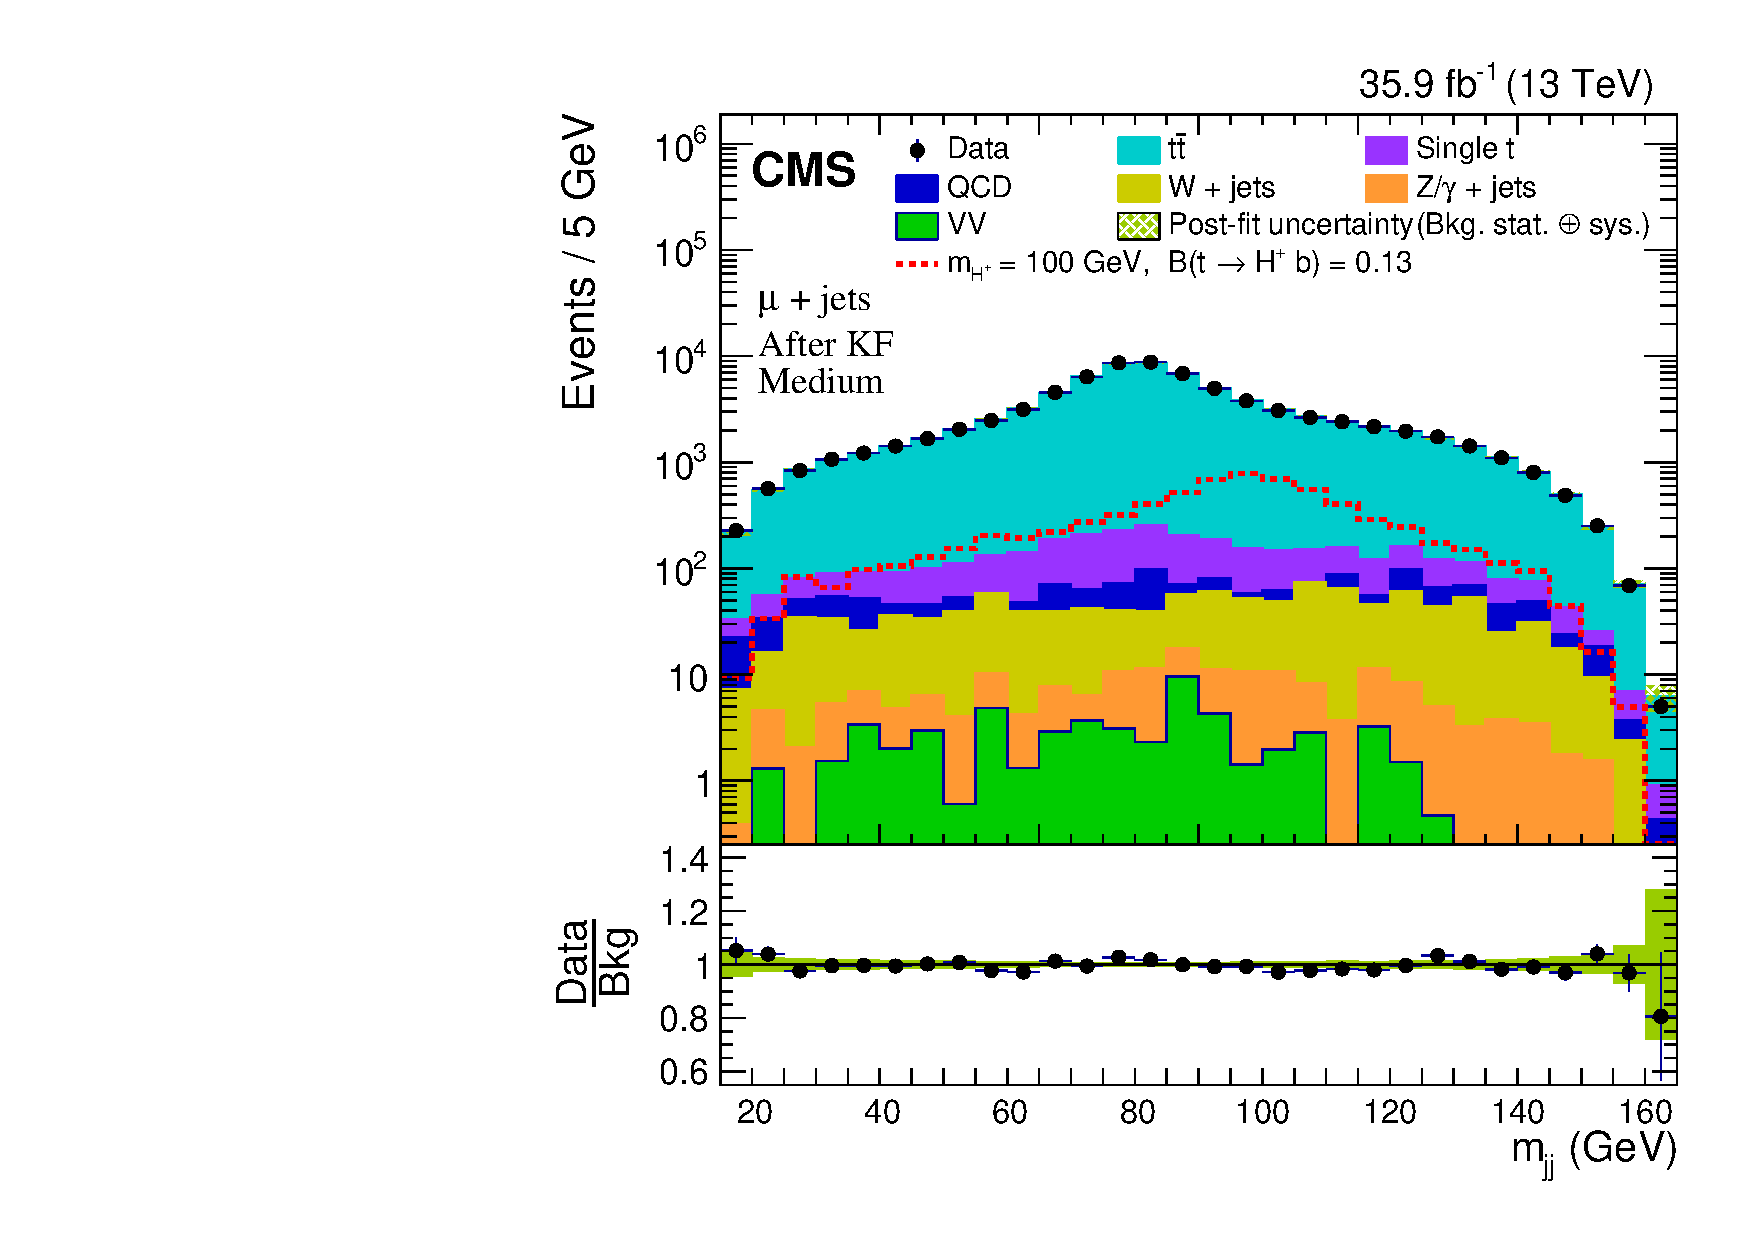
\includegraphics[width=0.45\textwidth]{Image/PostFit/mjj_postfit_ch2.pdf}}
{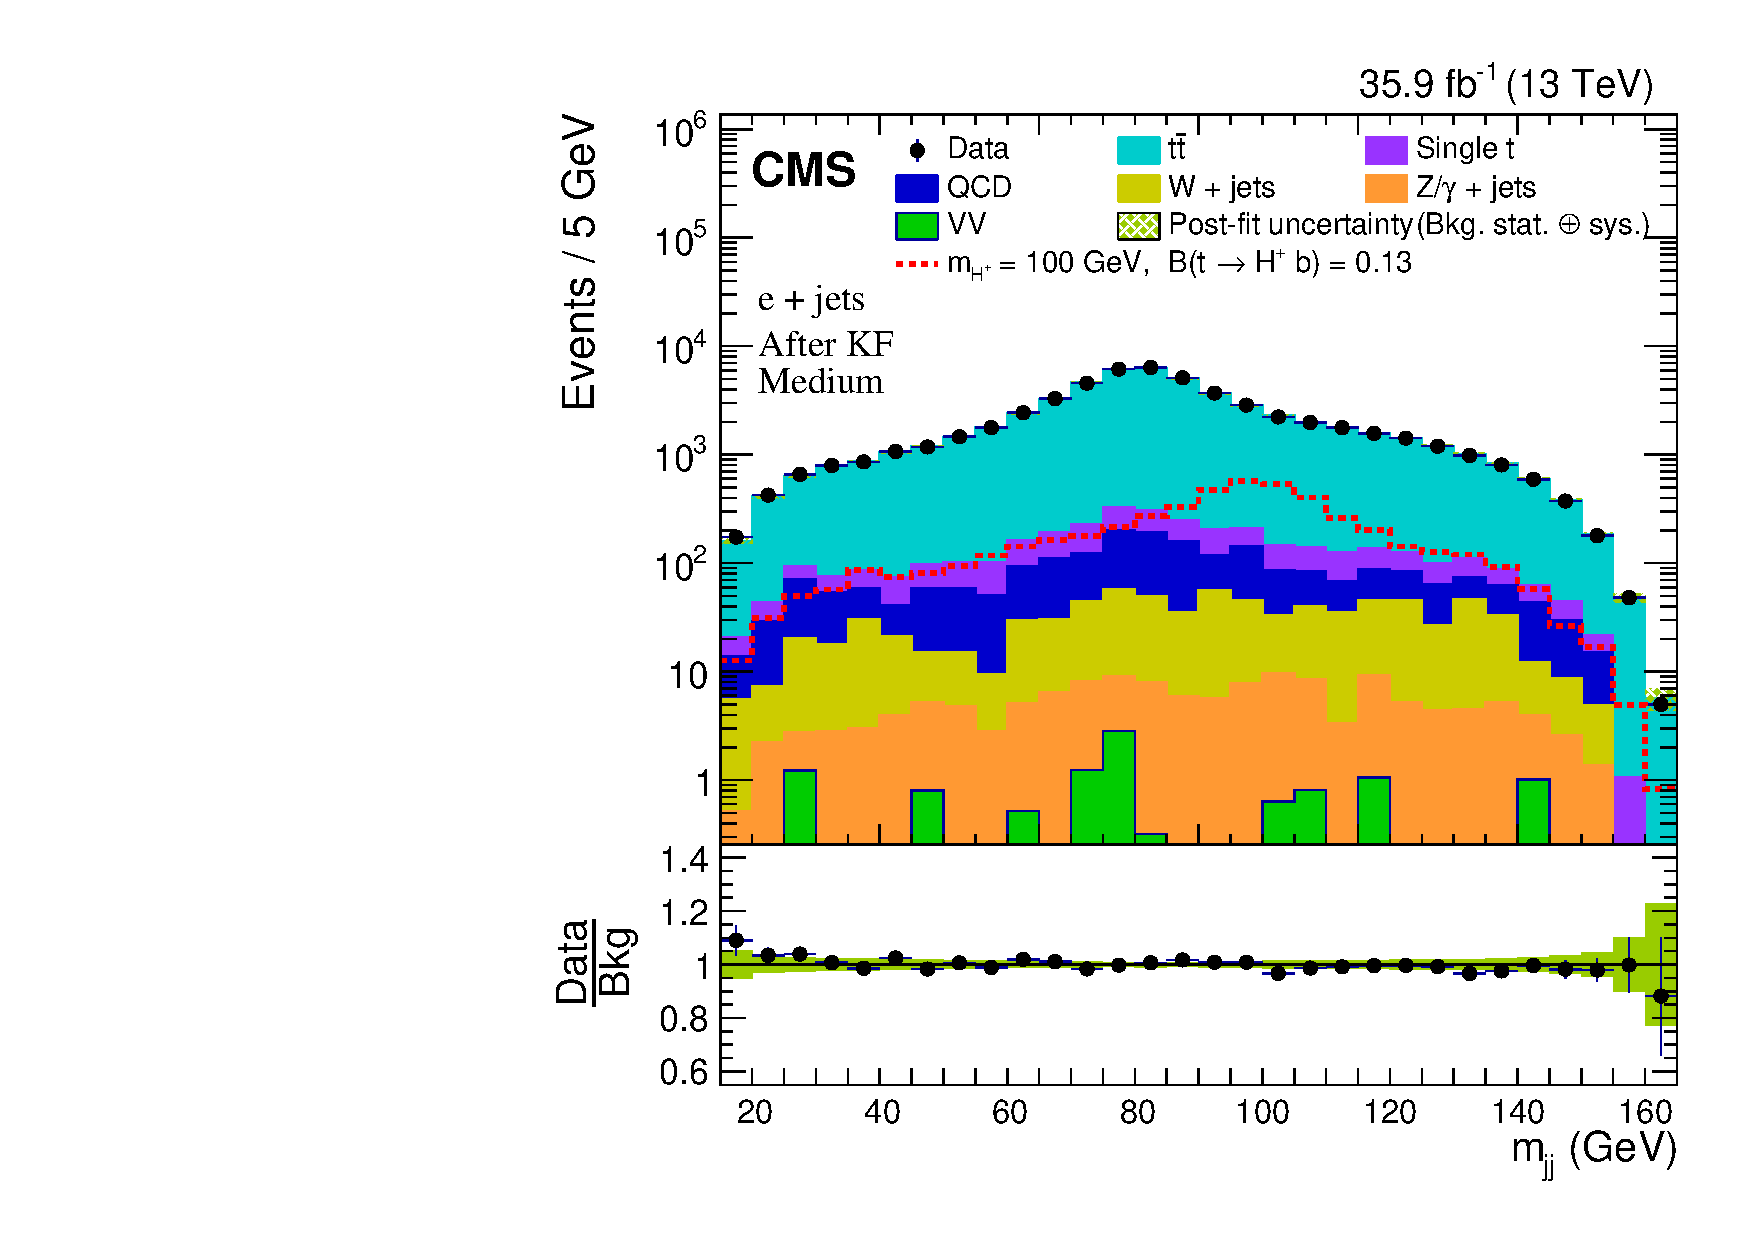
\includegraphics[width=0.45\textwidth]{Image/PostFit/mjj_postfit_ch5.pdf}}
{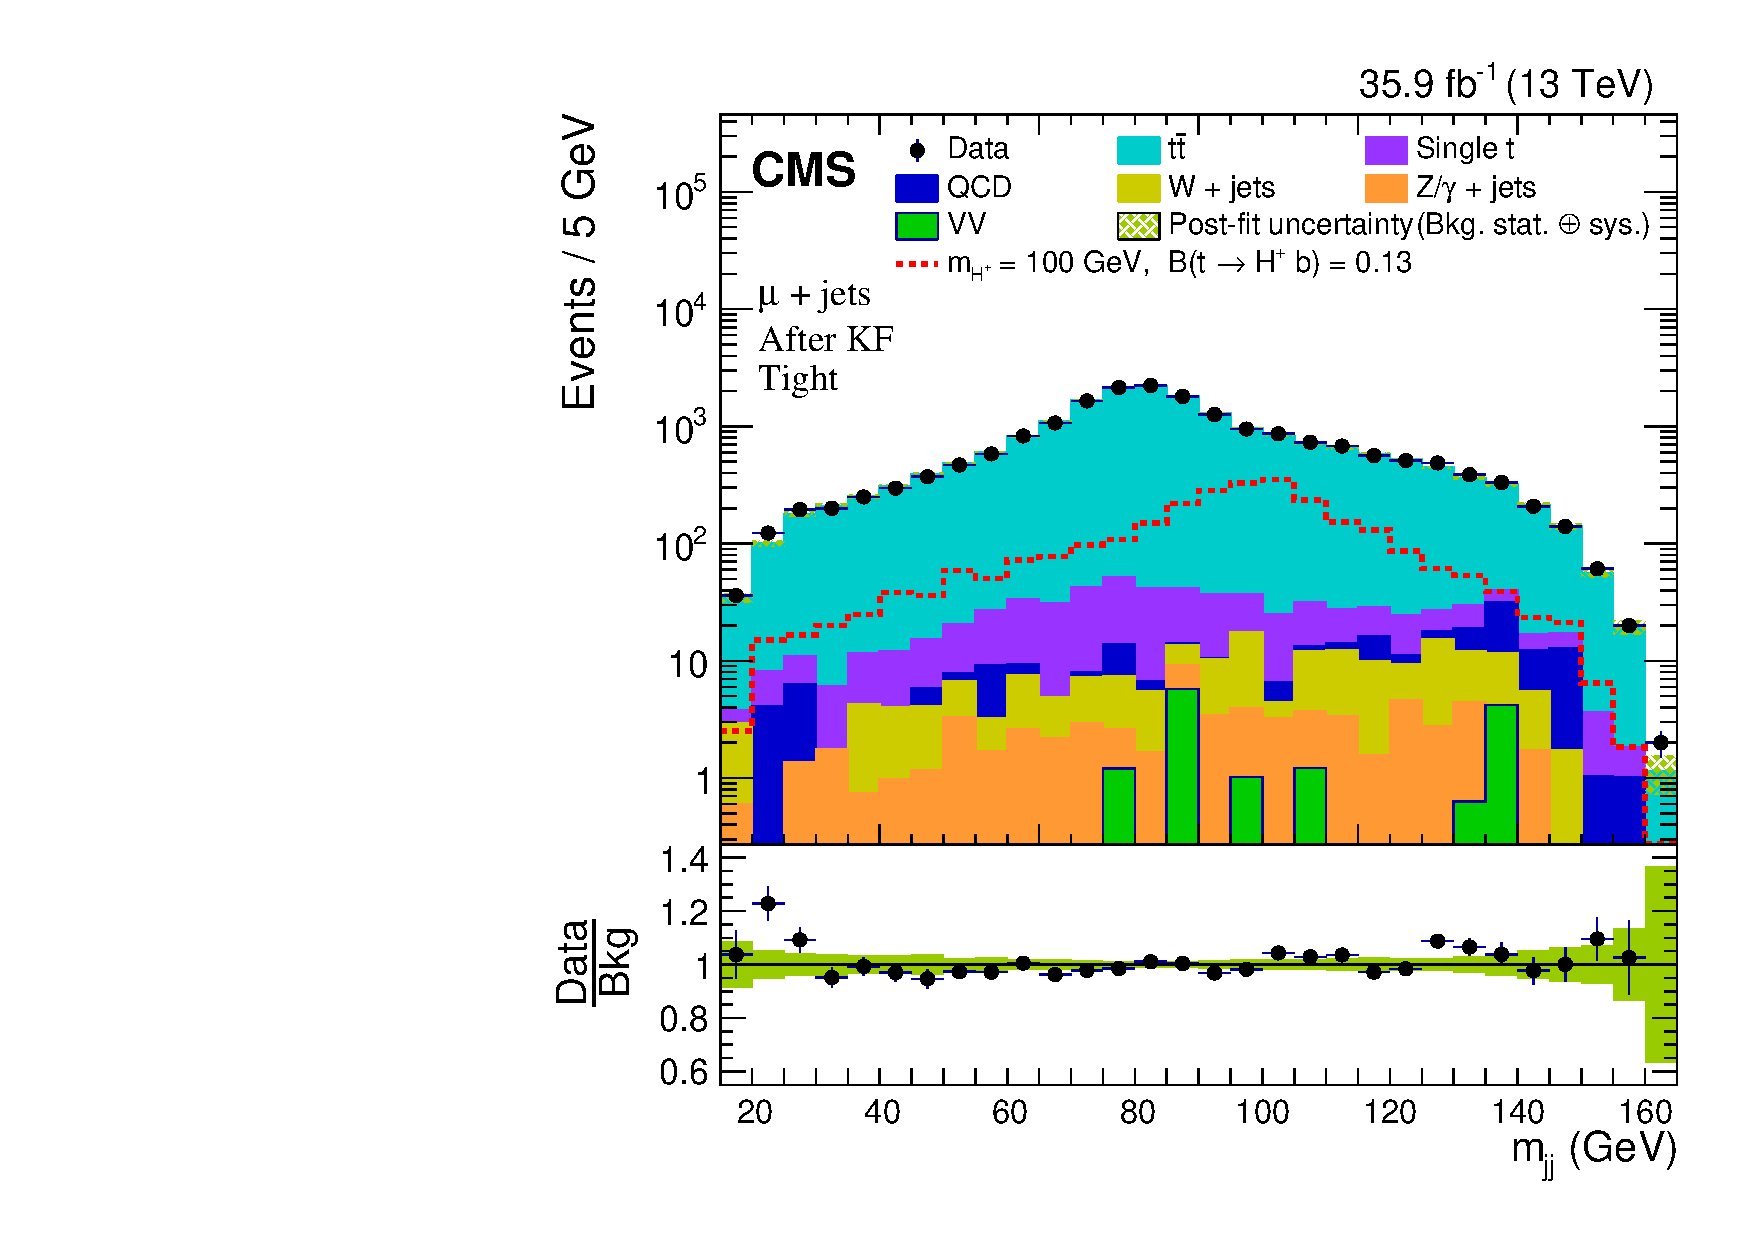
\includegraphics[width=0.45\textwidth]{Image/PostFit/mjj_postfit_ch3.pdf}}
{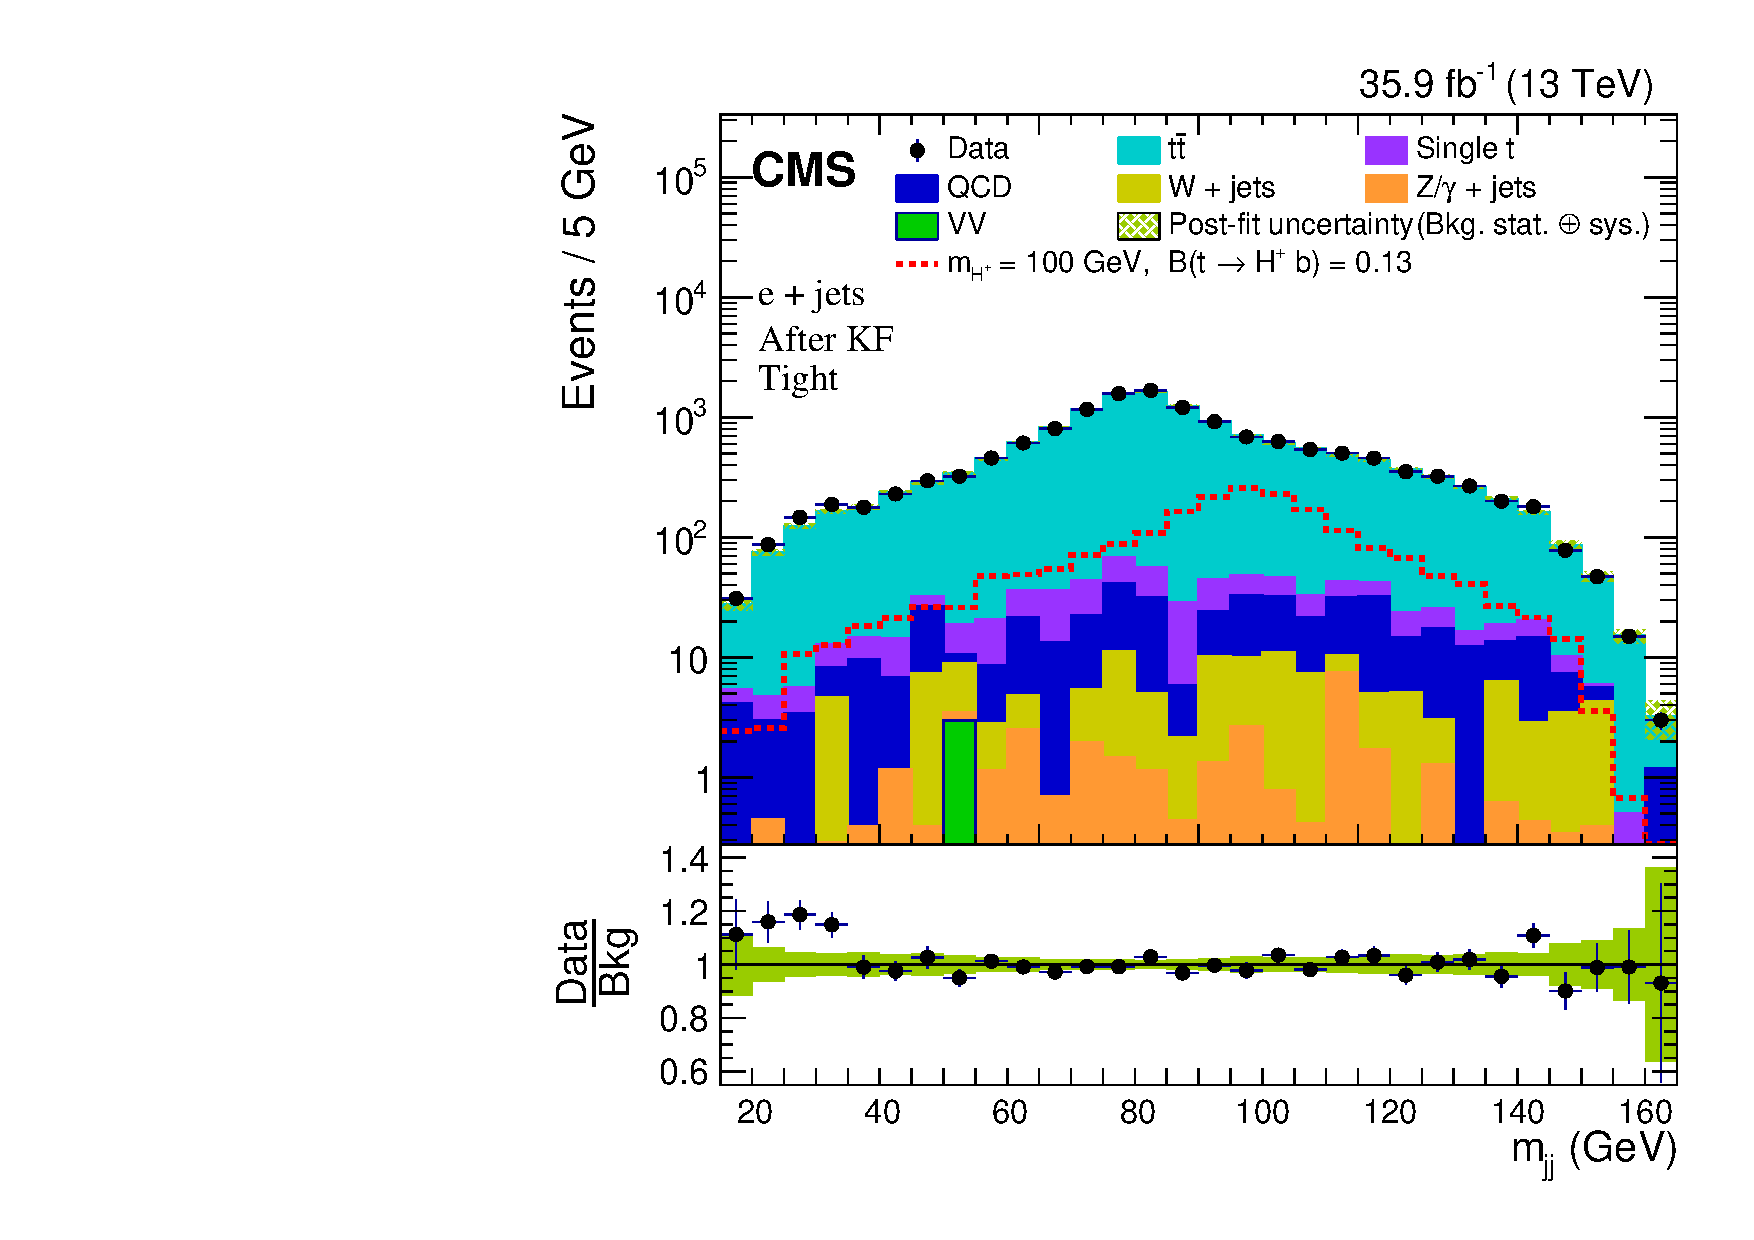
\includegraphics[width=0.45\textwidth]{Image/PostFit/mjj_postfit_ch6.pdf}}
\caption{Post-fit distributions of $\mjj$ from the exclusive charm
    categories for the \mujets (left column) and \ejets
    (right column) channel. The upper row shows the exclusive loose category,
    the middle row shows the exclusive medium category, and the lower row
    shows the exclusive tight category. The uncertainty band includes
    statistical as well as systematic uncertainties. The expected signal is
    shown prior to the fit to data.}
\label{fig:mjjPostFit}
\end{figure}
\begin{figure}
\centering
{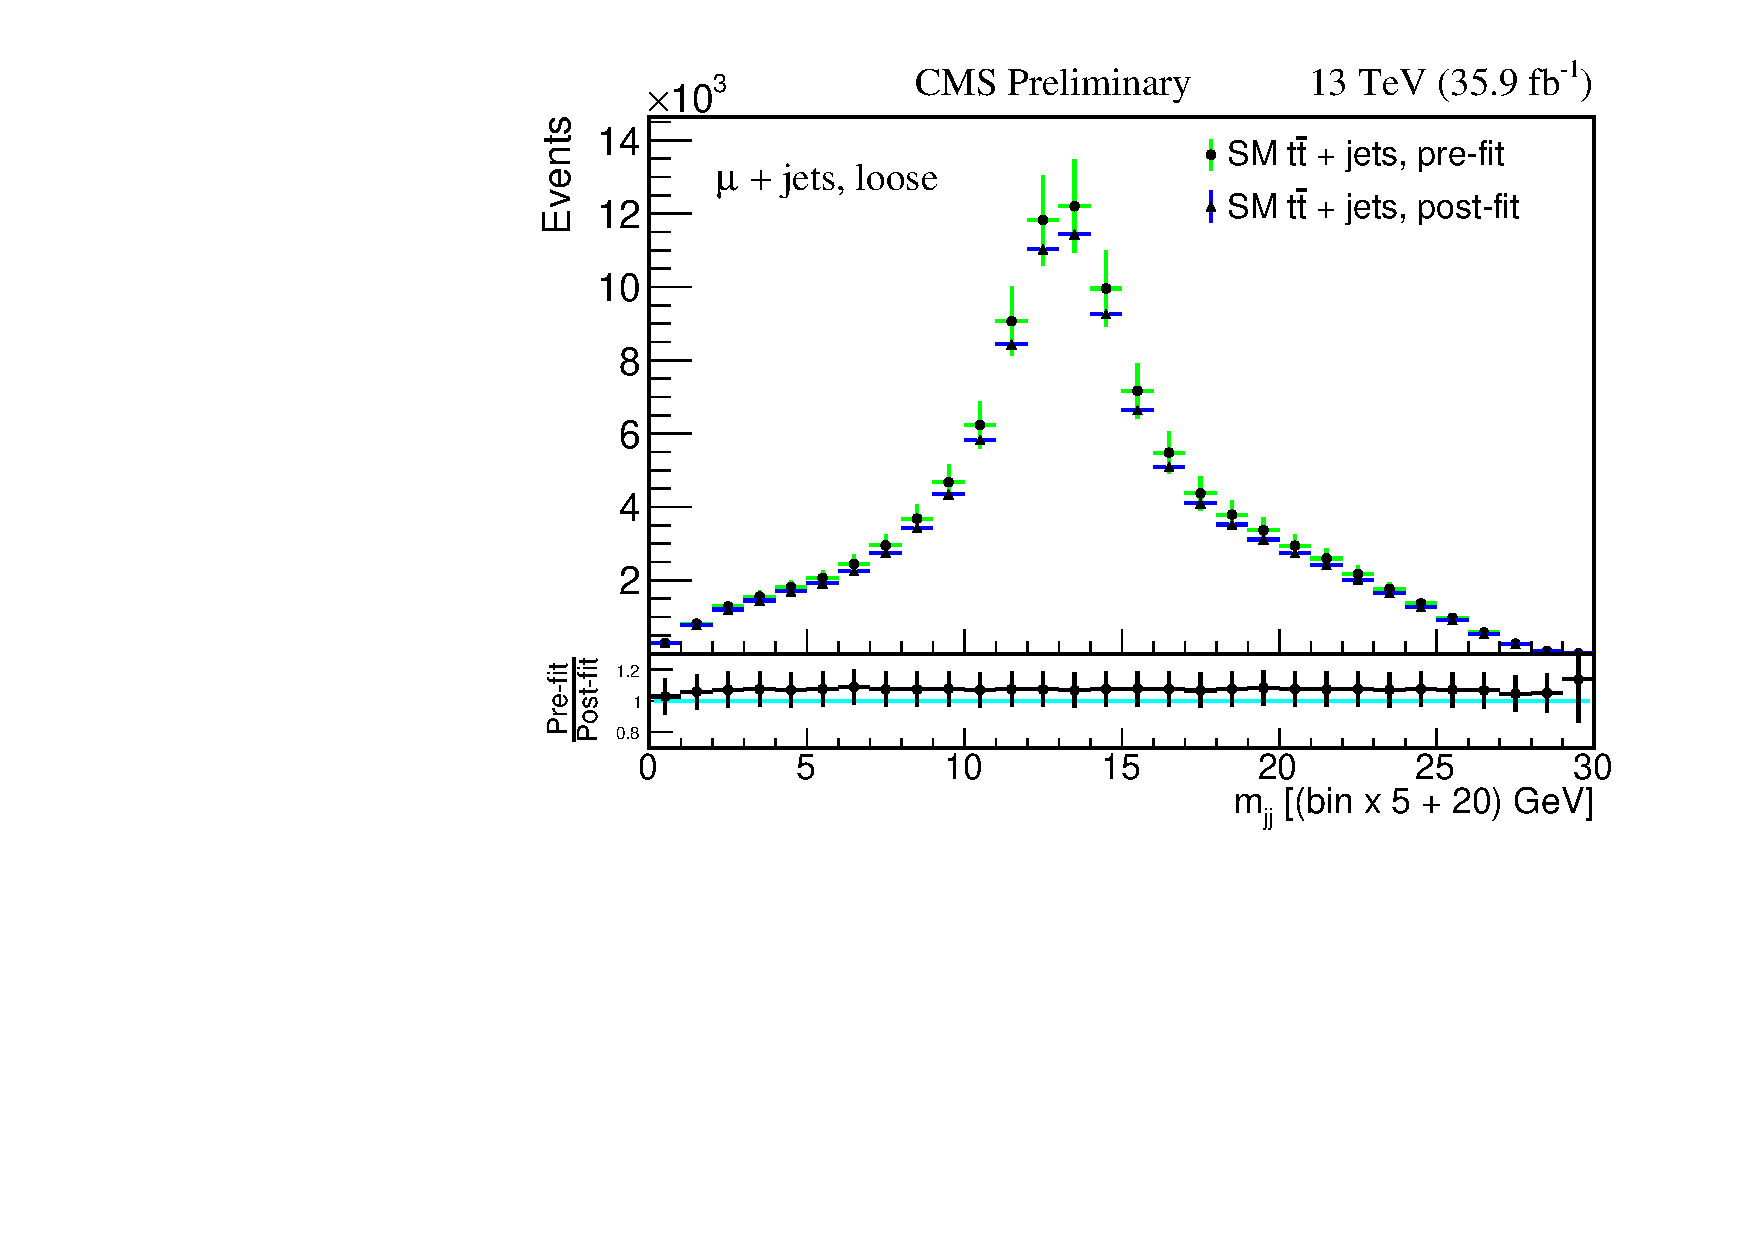
\includegraphics[width=0.49\textwidth]{Image/PostFit/ttbarPostFit_ch1.pdf}}
{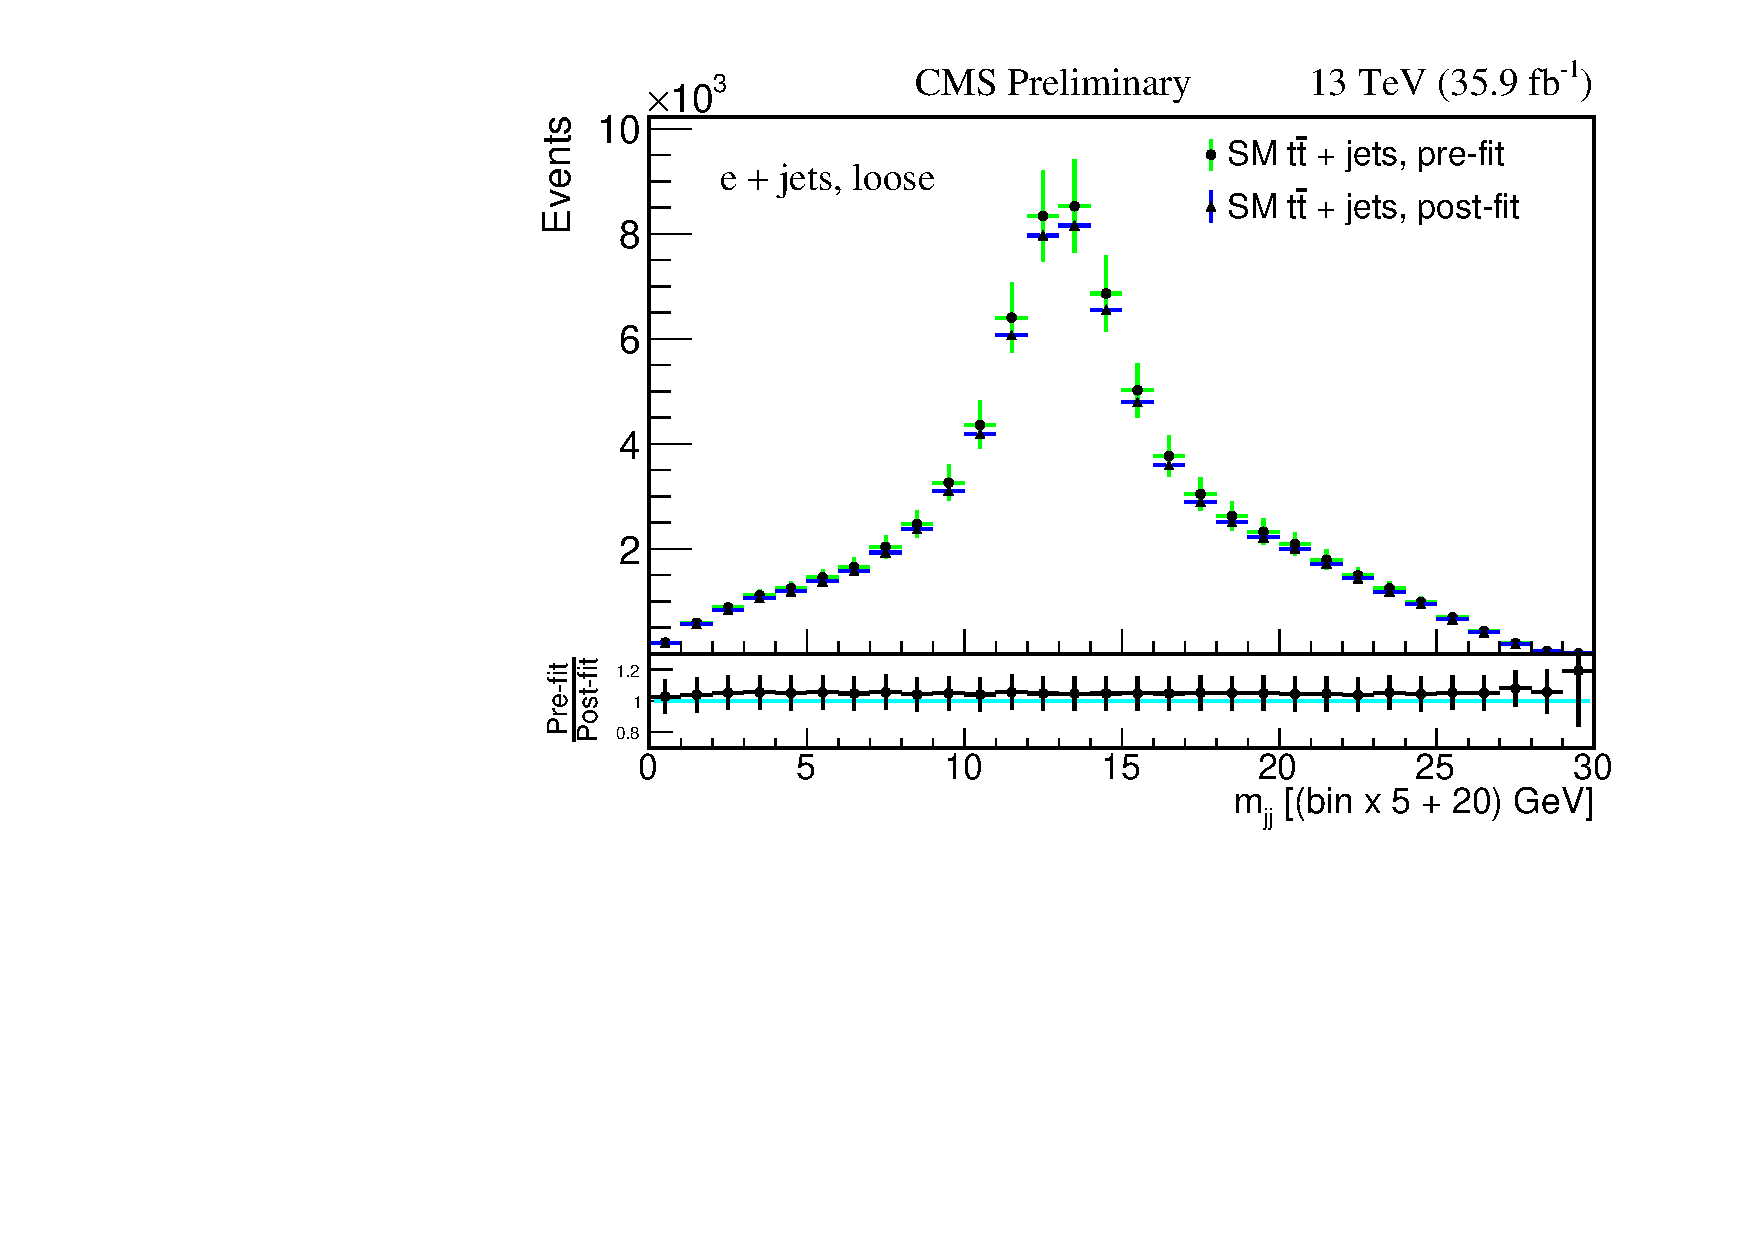
\includegraphics[width=0.49\textwidth]{Image/PostFit/ttbarPostFit_ch4.pdf}}
{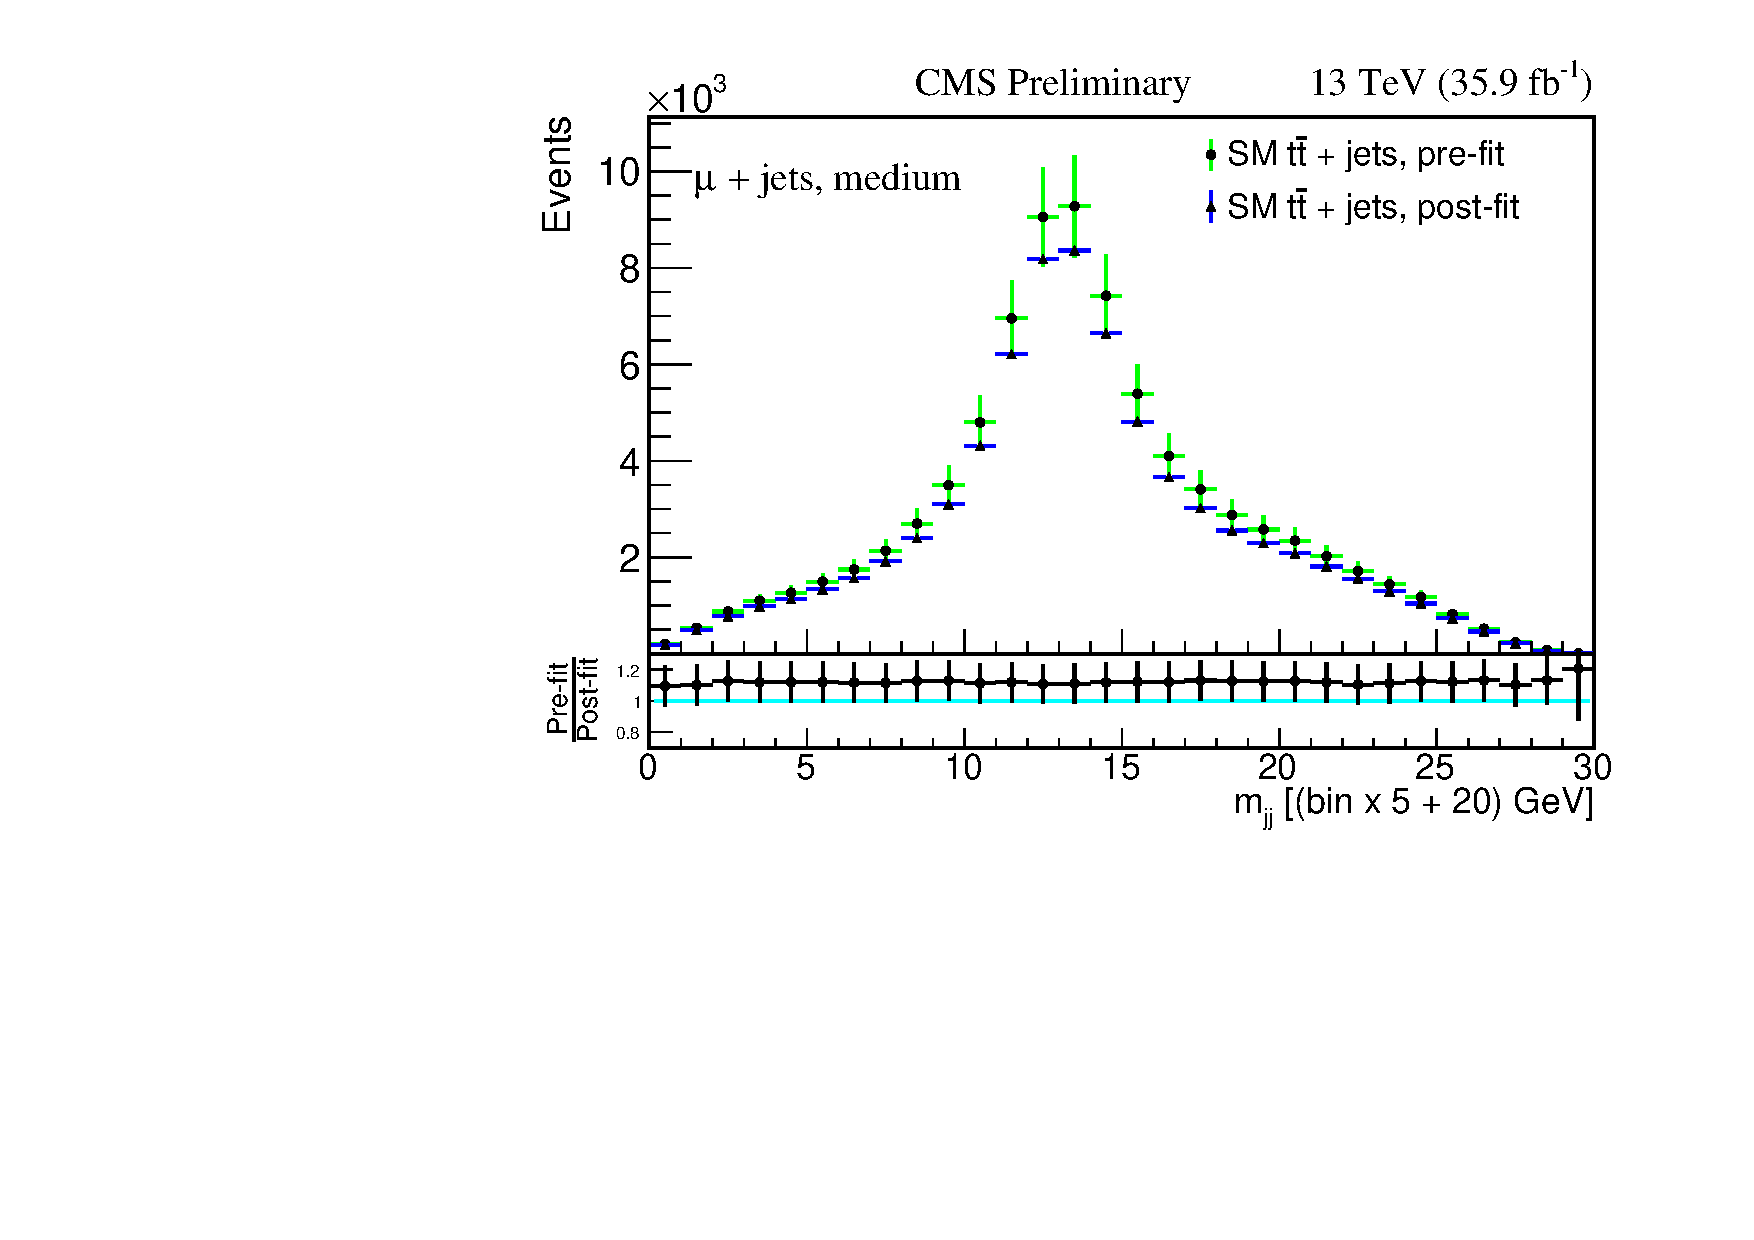
\includegraphics[width=0.49\textwidth]{Image/PostFit/ttbarPostFit_ch2.pdf}}
{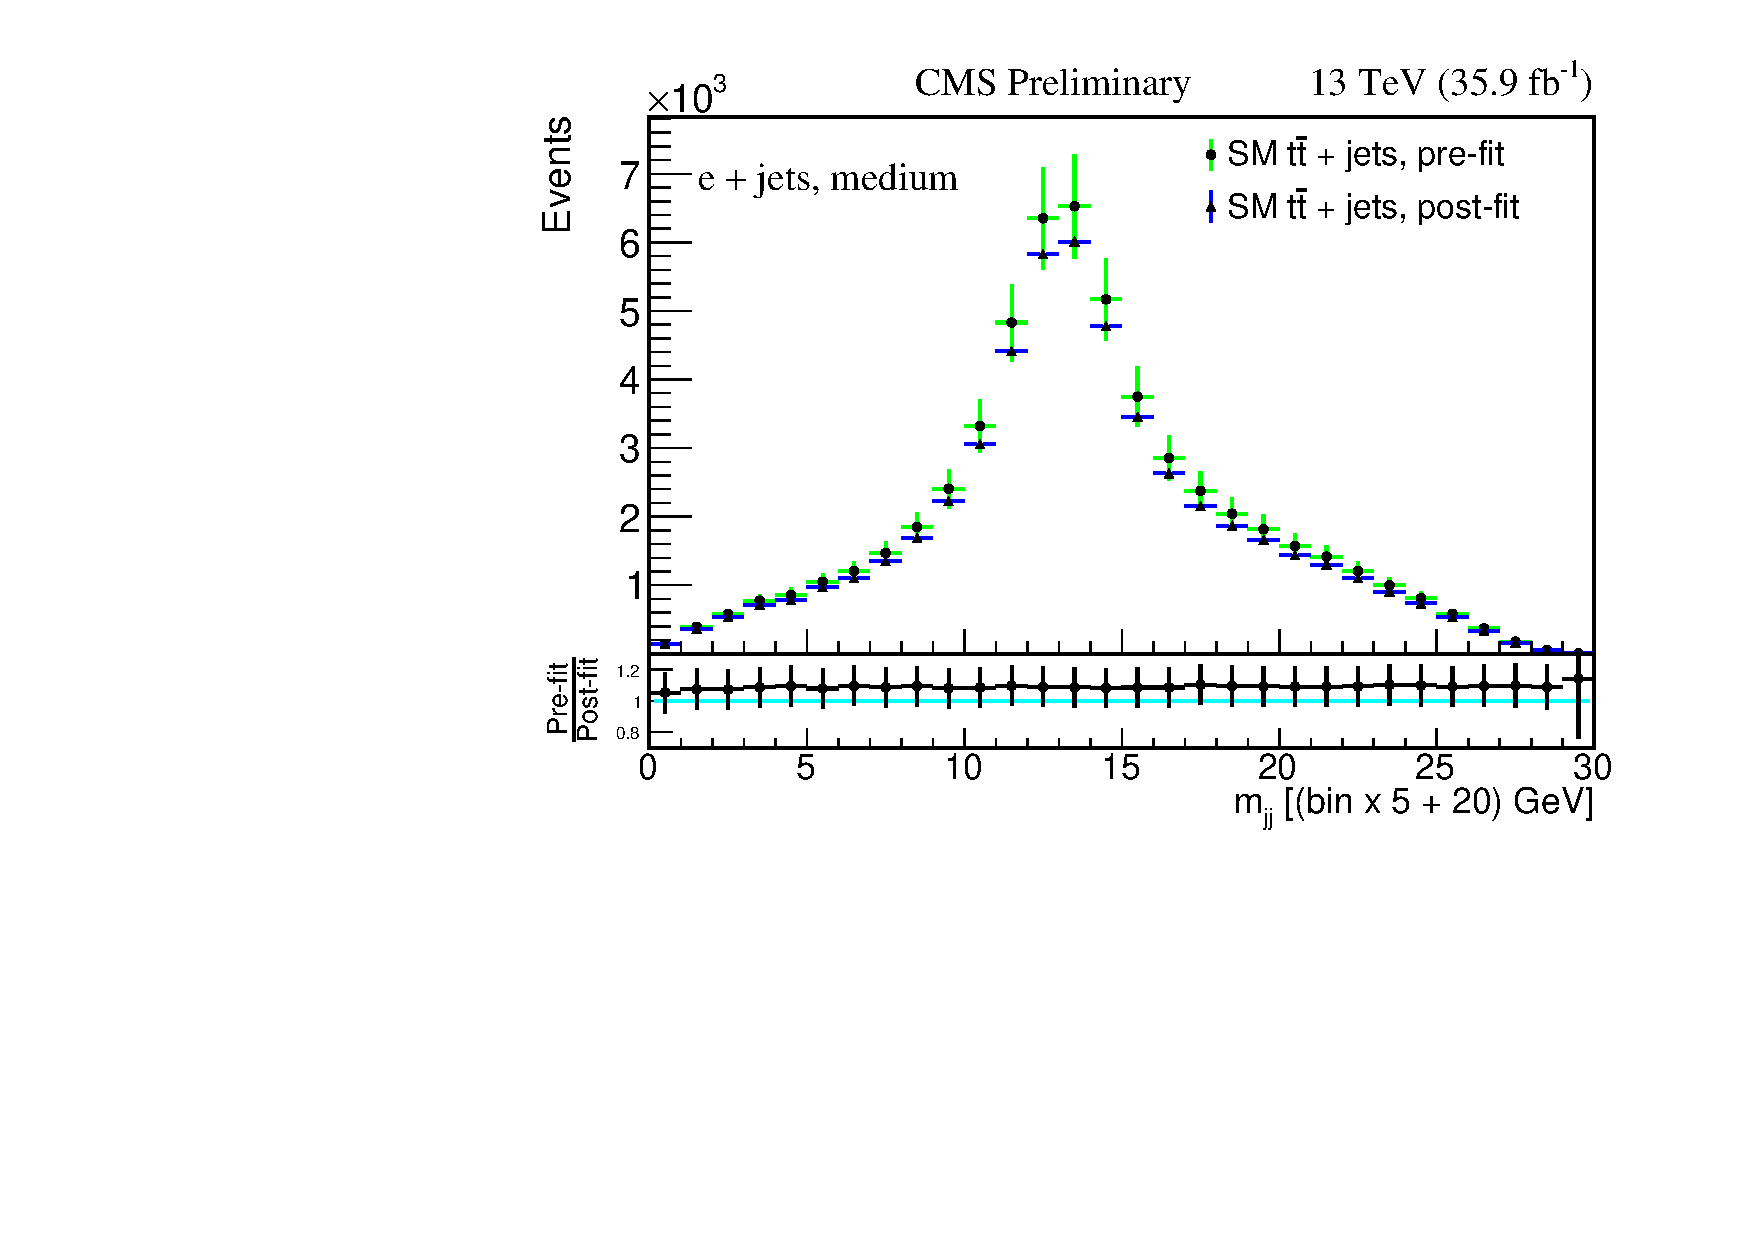
\includegraphics[width=0.49\textwidth]{Image/PostFit/ttbarPostFit_ch5.pdf}}
{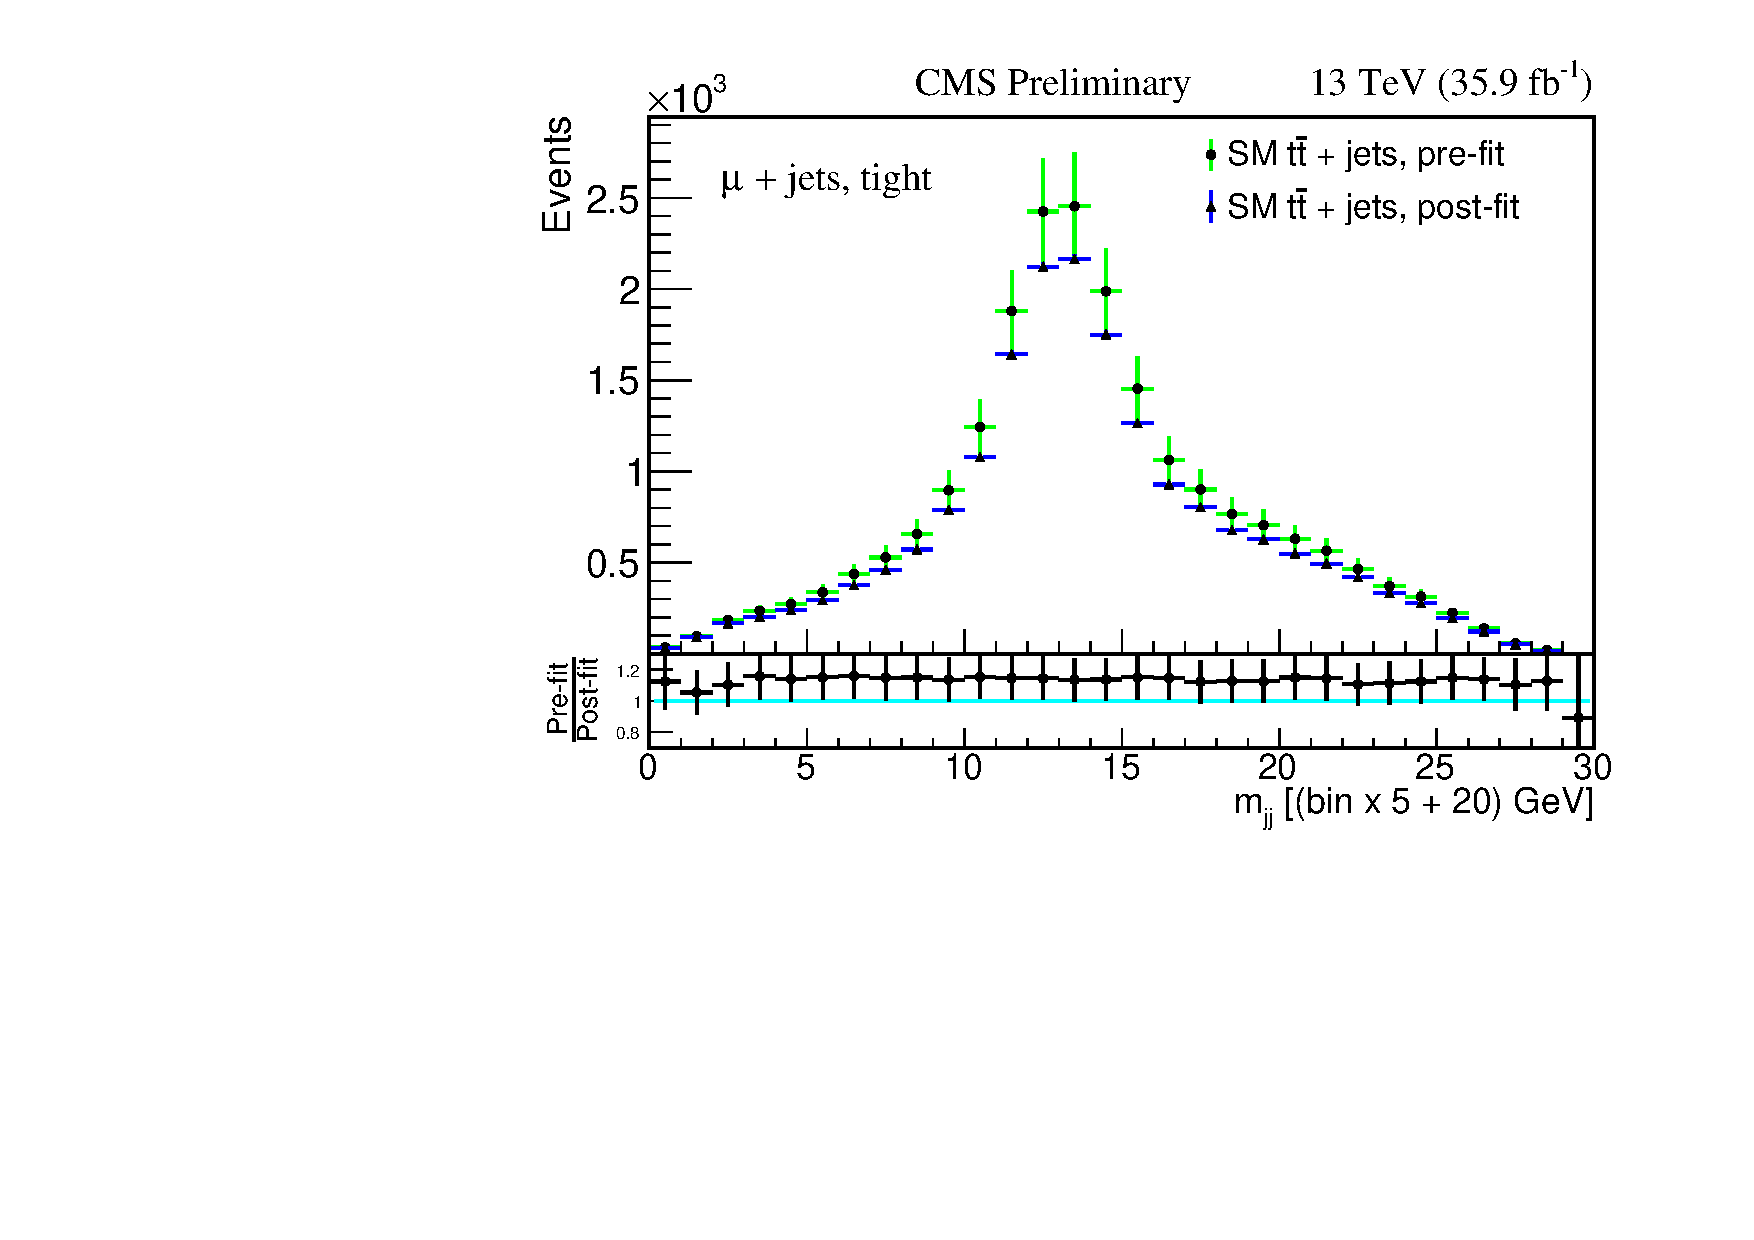
\includegraphics[width=0.49\textwidth]{Image/PostFit/ttbarPostFit_ch3.pdf}}
{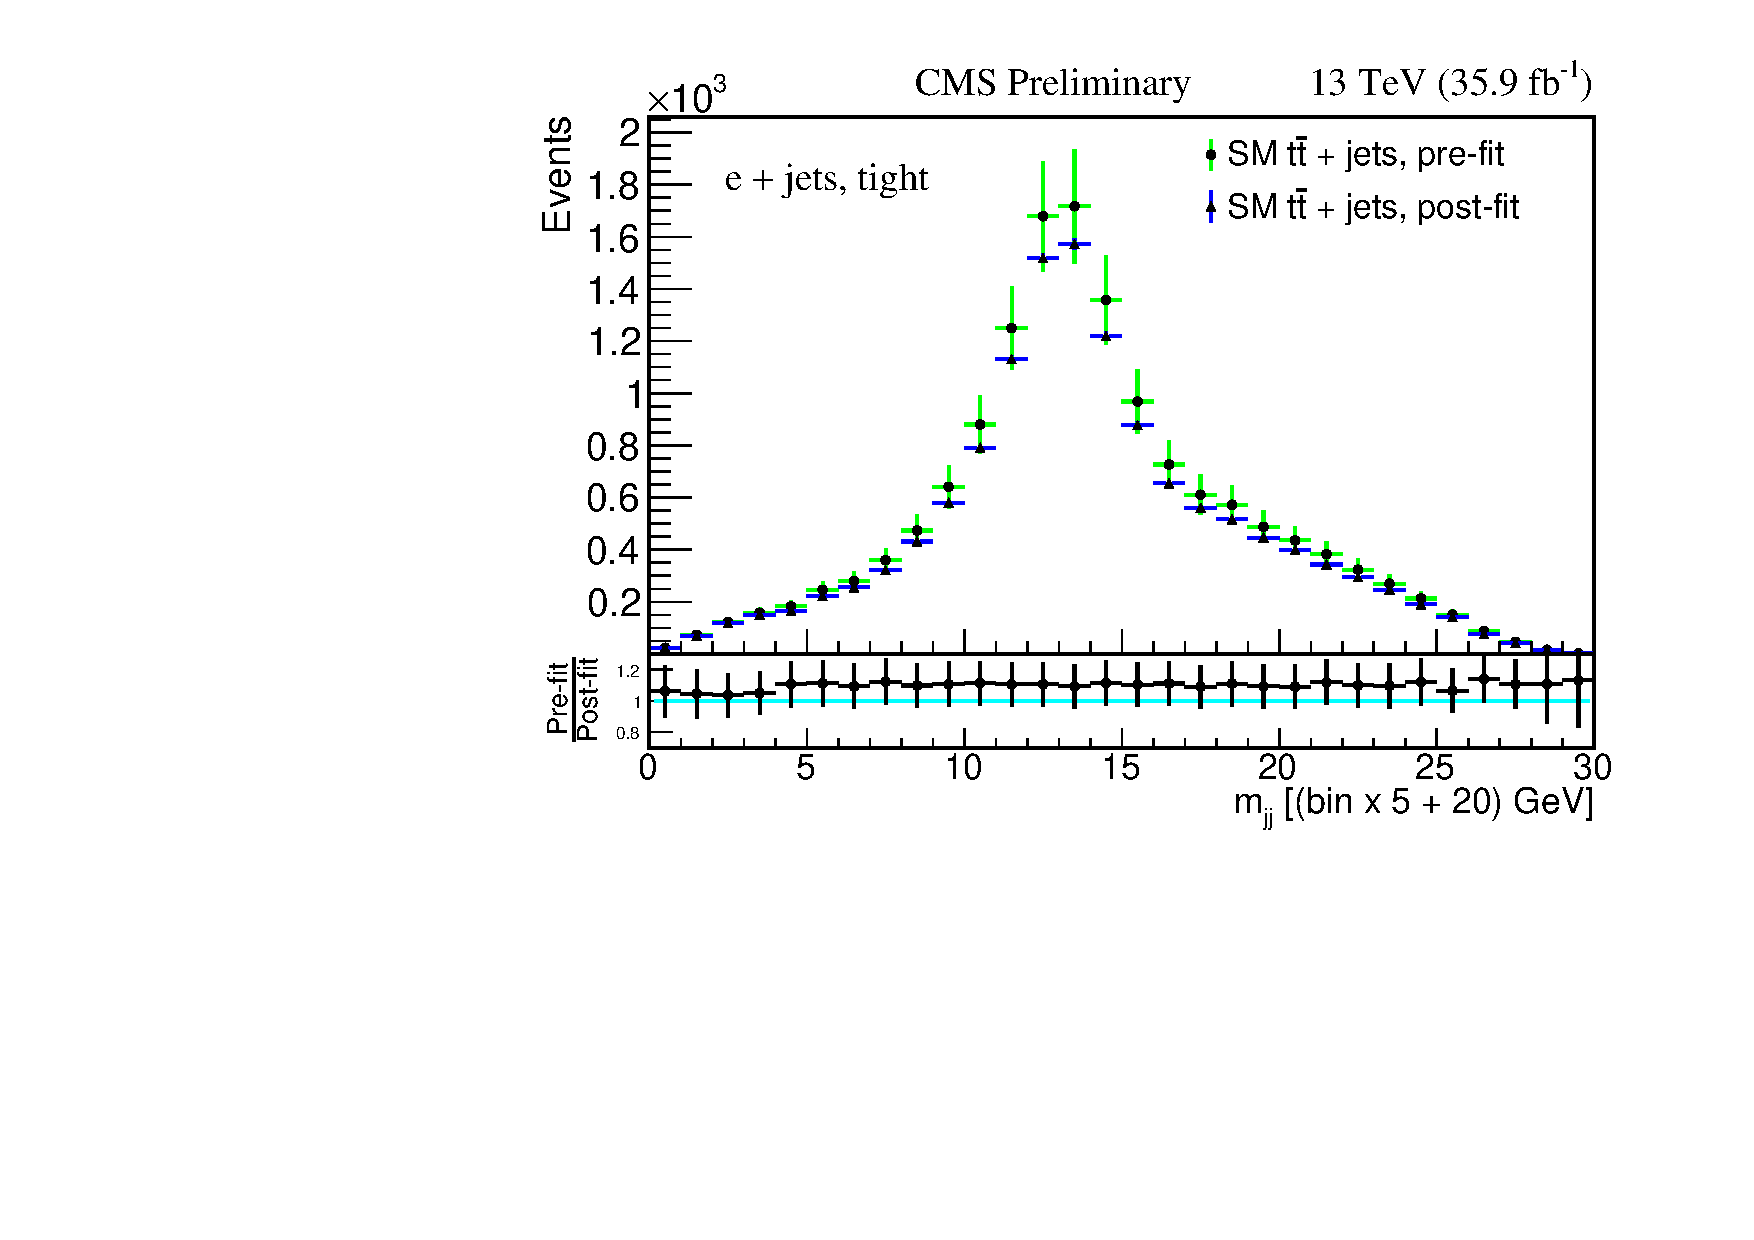
\includegraphics[width=0.49\textwidth]{Image/PostFit/ttbarPostFit_ch6.pdf}}
\caption{Pre-fit and post-fit distributions of $\mjj$ from SM $\ttjets$
    background for the exclusive charm categories for the \mujets
    (left column) and \ejets (right column) channel. The upper row
    shows the exclusive loose category, the middle row shows the exclusive
    medium category, and the lower row shows the exclusive tight category.
    The uncertainty includes statistical as well as systematic uncertainties.}
\label{fig:ttbarPostFit}
\end{figure}

\subsection{Corelation Among the Nuisance Parameters}
The reduction in the post-fit uncertainty can not be explained by looking
at the post-fit values of nuisance parameters shown in
Figures~\ref{fig:fitDiag1}-\ref{fig:fitDiag4}. If the NPs are very tightly
constrained then the post-fit uncertainty is expected to be heavily reduced.
However, that is not the case. Reductions in the post-fit uncertainty are not
only caused by constraints on the nuisance parameters, but also by
anti-correlations between the parameters. The size of the reduction can be quite
different for the different background processes because these processes are not
always affected by the same nuisance parameters, and even when the same nuisance parameter applies to different processes, the effect on the yield is not always the same.

The correlation among the leading nuisance parameters is shown in
Figure~\ref{fig:CorelationNP}. From this figure, it can be seen that there is
a large anti-correlation among the NPs. We also have positive correlations.
Therefore, the final uncertainty which is computed by taking into account
all the correlations is reduced after the post-fit. Note that, the pre-fit
uncertainties are either positively-correlated or not correlated at all among
themselves.

%\begin{figure}
\begin{sidewaysfigure}
\centering
{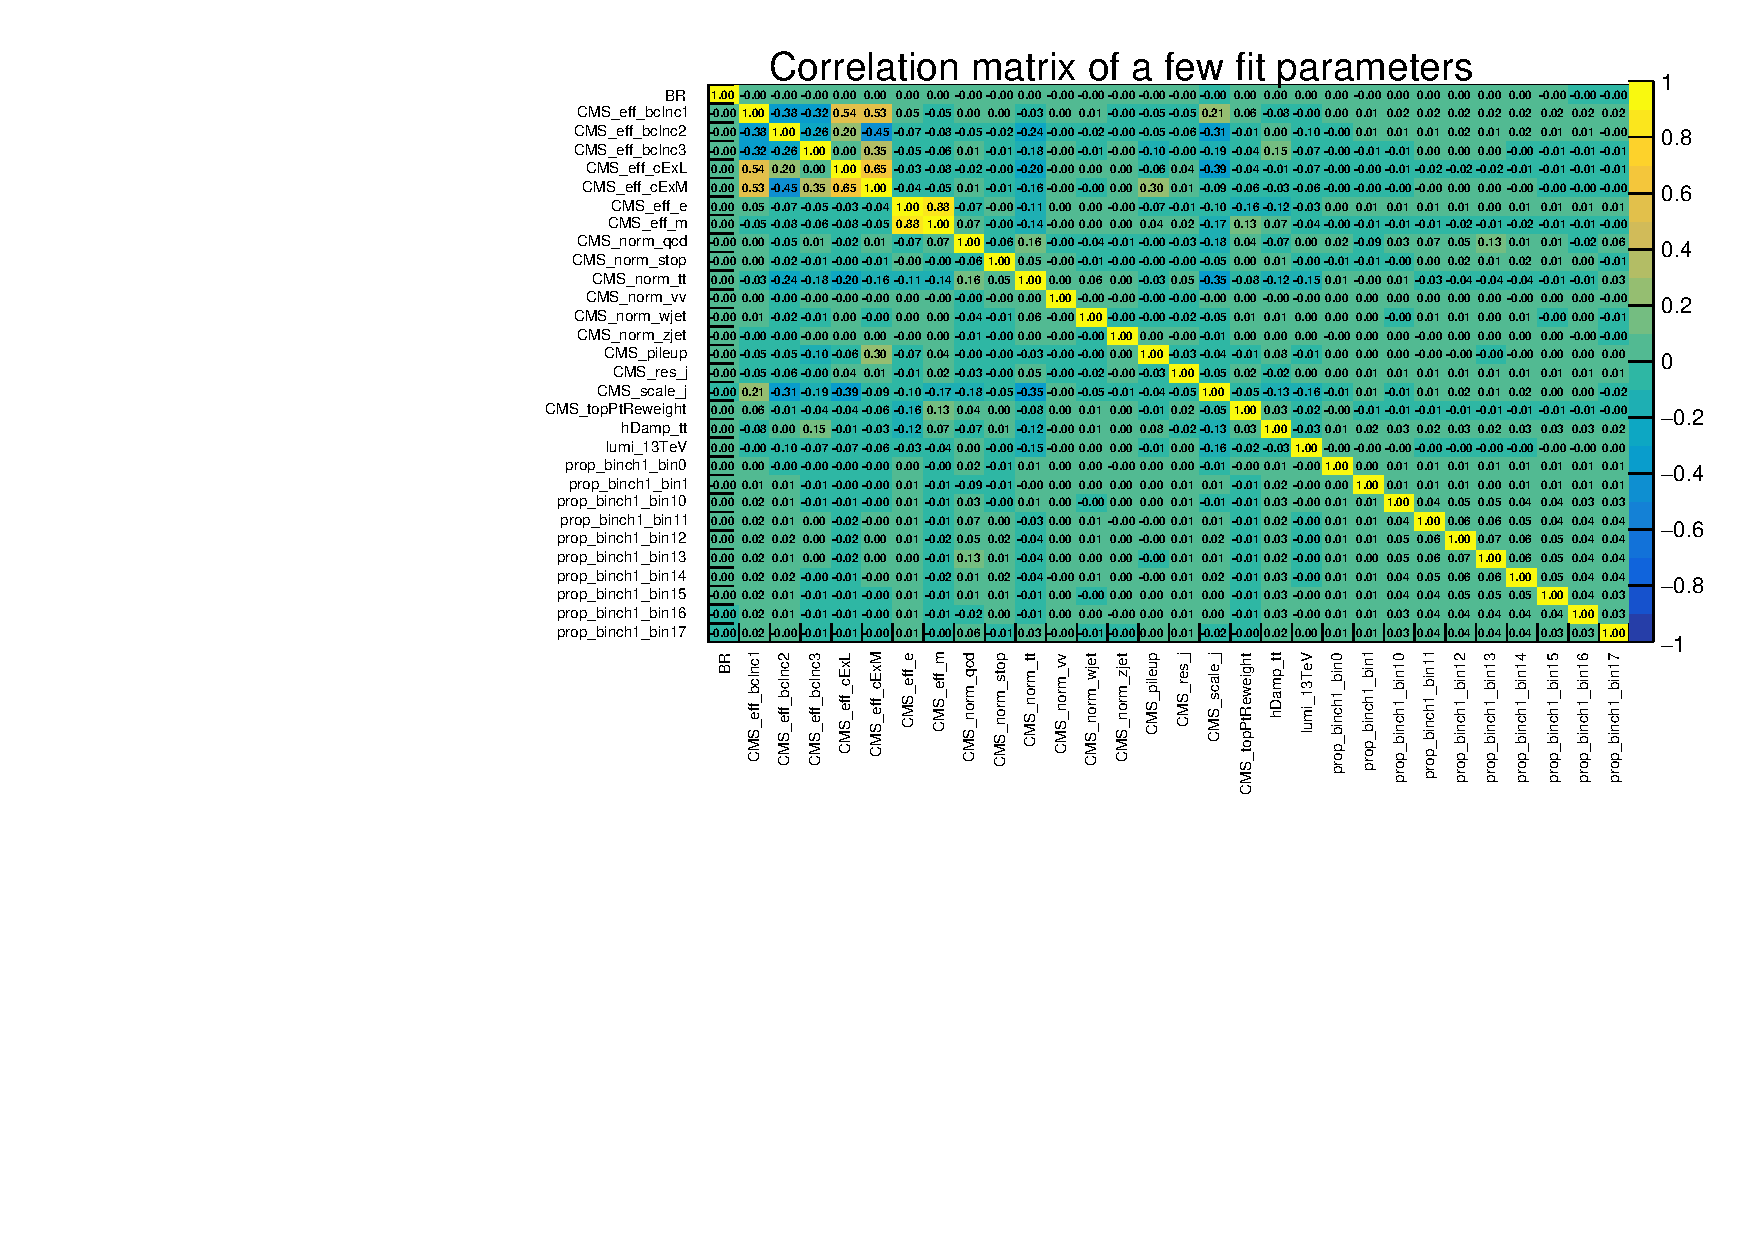
\includegraphics[width=1.0\textwidth]{Image/PostFit/CorelationNP.pdf}}
\caption{Correlation among the leading NPs for \ljets channel, $m_{H^+} = 100$ GeV. All the systematics and a few statistical NPs are shown. The systematic
NPs have positive as well as negative correlation with other NPs. However, the
statical NPs are mostly positively correlated.}
\label{fig:CorelationNP}
%\end{figure}
\end{sidewaysfigure}
